\documentclass[a4paper,fleqn]{cas-dc}

\usepackage[numbers,sort&compress]{natbib}
\usepackage{amsmath,amssymb}
\usepackage{booktabs}
\usepackage{graphicx}
\usepackage{multirow}
\usepackage{placeins}
\usepackage{tabularx}
\usepackage{xcolor}
\usepackage{url}
\usepackage{hyperref}

\graphicspath{{../assets/figures/}}
\setlength{\emergencystretch}{2em}
\newcolumntype{Y}{>{\raggedright\arraybackslash}X}
% The source argument preserves one-to-one evidence mapping; the typeset
% draft uses a compact marker.
\newcommand{\TBD}[1]{\textcolor{red!70!black}{\textbf{TBD}}}
\newcommand{\query}{\texttt{descriptor\_}\allowbreak\texttt{cheap}}
\newcommand{\DBF}{Decision-before-Feature}

\begin{document}
\let\WriteBookmarks\relax
\def\floatpagepagefraction{1}
\def\textpagefraction{.001}

\shorttitle{Decision before Feature in Black-box Optimization}
\shortauthors{Anonymous Author(s)}

\title[mode=title]{Decision before Feature: Deciding Whether to Execute a
Landscape Descriptor Query in Black-box Optimization}

\author[1]{Anonymous Author(s)}
\affiliation[1]{organization={Affiliation withheld for anonymous review},
                country={}}

\begin{abstract}
Landscape descriptors are widely used to support algorithm selection in
black-box optimization, but acquiring them consumes function evaluations,
runtime, and memory, while their value may vary across search states.  This
paper formulates acquisition of a fixed landscape-descriptor query as a
decision that precedes feature computation.  The proposed \DBF{} protocol
reuses algorithm-agnostic,
permutation-invariant behavior from complete native optimizer-update histories,
constructs state-aligned query-utility labels through paired offline
continuations, and freezes a supervised decision rule under nested
function-family out-of-fold evaluation.  The primary query is a predefined
16-dimensional low-cost descriptor configuration; two larger configurations
are reserved for representation-and-cost sensitivity analyses.
\TBD{TBD-ABS-RQ1}
The prevalence and interval for non-beneficial primary-query states remain
undetermined.
\TBD{TBD-ABS-RQ2}
The nested-OOF model comparison, frozen held-out BBOB-family evaluation, and
B3-versus-T0 increment remain undetermined.
\TBD{TBD-ABS-RQ3}
The end-to-end comparison with the prespecified baselines, including query
use, final performance, and resource measures, remains undetermined.
\TBD{TBD-ABS-RQ4}
Performance on BBOB validation, CEC2017, CEC2022, and engineering problems
remains undetermined; no transfer claim is made.
\TBD{TBD-ABS-RQ5}
The association between search behavior, search maturity, and query utility
remains undetermined and has a descriptive, non-causal interpretation.
\end{abstract}

\begin{highlights}
\item Formulates landscape-descriptor acquisition as a decision made before
      descriptor computation.
\item Uses offline, state-aligned utility labels and algorithm-agnostic search
      behavior from native optimizer histories.
\item Specifies train-only model selection and threshold freezing before any
      held-out benchmark evaluation.
\end{highlights}

\begin{keywords}
black-box optimization \sep algorithm selection \sep landscape analysis \sep
trajectory features \sep resource-aware decision making \sep function-family
generalization
\end{keywords}

\maketitle

\section{Introduction}
\label{sec:introduction}

Black-box optimization is used when objective values can be obtained by evaluation but an analytic model, derivative information, or a tractable problem structure is unavailable. In this setting, the choice of optimizer matters: algorithms expose complementary behavior across problem instances, while no member of a practical portfolio is uniformly preferable. Automated algorithm selection addresses this heterogeneity by mapping an instance representation to a portfolio decision. A common workflow evaluates a space-filling design, computes exploratory landscape analysis (ELA) features, and then applies a supervised selector \cite{kerschkeAutomatedAlgorithmSelection2019,guoAutomatedAlgorithmSelection2025}. This workflow makes landscape analysis a prerequisite for selection.

That prerequisite is not innocuous. Landscape characterization comprises families of measures with different assumptions, sampling requirements, search dependence, and computational demands \cite{malanSurveyTechniquesCharacterising2013,pragerPflaccoFeaturebasedLandscape2024}. The objective evaluations used to construct a landscape sample consume budget that could otherwise be assigned to optimization, and the appropriate feature-computation fraction depends on the selection scenario \cite{blomInfluenceFeatureComputation2026}. Contemporary systems therefore count feature evaluations or omit expensive groups under a restricted budget \cite{guoAutomatedAlgorithmSelection2025}. An ELA-informed portfolio decision may be useful and still fail to justify the resources spent to obtain its descriptors at a particular search state.

At the same time, an optimization prefix already produces information. Search-trajectory networks characterize convergence patterns, recurrent transitions, and attraction regions from ordinary optimizer runs \cite{ochoaSearchTrajectoryNetworks2021}. DynamoRep preserves the longitudinal evolution of population summaries, while Opt2Vec learns from populations visited during search \cite{cenikjDynamoRepTrajectoryBasedPopulation2023,korosecOpt2VecContinuousOptimization2024}. Probing trajectories use short objective-value sequences for a subsequent portfolio choice, and later work shows that their evaluation depends on both the classifier and the problem-level split \cite{renauUtilityProbingTrajectories2024,renauAlgorithmSelectionProbing2025b}. Reusing evaluated points avoids a separate objective-function sample, but representation and inference still have computational cost. More importantly, problem classification or direct algorithm selection does not establish that a pre-query behavior summary predicts the net value of acquiring an independent descriptor query.

Generalization is a second obstacle. Algorithm-selection performance can appear strong when training and evaluation sets contain closely related instances. Under demanding problem and problem-combination splits, several classical and learned landscape representations did not improve over a single-best-solver baseline in the evaluated affine-BBOB setting \cite{cenikjLandscapeFeaturesSingleobjective2025}. The closest per-run warm-starting study likewise reported that results obtained on BBOB did not transfer directly to YABBOB \cite{kostovskaPerrunAlgorithmSelection2022}. Recent reviews identify heavy reliance on BBOB, heterogeneous feature protocols, and limited cross-benchmark evidence as continuing concerns \cite{cenikjSurveyFeaturesUsed2026}. Random instance partitions and within-training scores are therefore insufficient evidence for transfer to unseen function families or benchmark suites.

This paper studies a decision that precedes feature acquisition: given an optimization prefix and its algorithm-agnostic behavioral history, should a fixed landscape-descriptor query be executed at the current state? We call this setting \emph{Decision-before-Feature}. It differs from trajectory-based per-run selection, which constructs a trajectory representation and chooses a second-stage algorithm \cite{jankovicTrajectorybasedAlgorithmSelection2022,kostovskaPerrunAlgorithmSelection2022}, and from dynamic algorithm selection, which repeatedly changes search actions during a run \cite{guoDeepReinforcementLearning2024b}. It also differs from landscape-aware operator or population control \cite{sallamLandscapebasedAdaptiveOperator2017,zhouAdaptiveMultipopulationArtificial2024}. The object here is not a parameter, operator, or optimizer update rule, but whether to acquire additional information before a downstream portfolio decision.

We formulate query value as the difference in clipped terminal $\log_{10}$ gap between a native no-query continuation and a query-plus-selector path from the same complete optimizer state, less a weighted $\log_{10}$ ratio of their state-to-terminal future-path runtimes. The primary time for each path is the median of three prespecified censored replays: a completed replay retains its observed time, whereas a timed-out or failed replay contributes the larger of its observed time and role-specific timeout. The already executed shared prefix is a sunk cost; full FE-zero-to-terminal wall-clock remains a separate policy endpoint. Memory is measured and reported separately in the primary analysis, for which $\lambda_M=0$. The query evaluations already reduce the remaining optimization budget and are not deducted twice. Query-sample evaluations do not enter the optimizer population, but their best point and observed target hit enter the operational Query endpoint. We distinguish an observed target hit, path completion, and completion-conditioned endpoint success; standard ERT uses the observed hit even when a later path failure occurs. Offline labels use fold-specific downstream selectors, whereas the deployed gate observes only behavior available before the query. Query descriptors, function identity, algorithm identity, optimizer-specific parameters, and known-optimum gaps are excluded from that gate. The resulting question is not whether landscape features can sometimes support selection, but when the expected downstream difference of the evaluated query is sufficient to justify its acquisition cost.

The study is organized around five research questions. RQ1 characterizes the statewise utility of the primary \query{} query. RQ2 tests whether algorithm-agnostic behavior adds decision value beyond elapsed budget and a dimension-stratified time-only comparator. RQ3 compares the resulting policy with fixed, random, traditional landscape-based, behavior-only, and portfolio references under common resource accounting. RQ4 reports the inspected six-function BBOB-validation set and CEC2017 as development evaluations, and reserves CEC2022 and engineering problems for prospective evaluation after their complete configurations and endpoints have been fixed. Each suite is reported separately. The BBOB-validation estimand is a finite-set mean, not a function-superpopulation or independent-confirmation estimand. RQ5 examines the six prespecified T0/B1/B2/B2+Motion/B2+Maturity/B3 groups, model-appropriate coefficient or discriminant stability, maturity--utility associations, and variation across function, dimension, and query configuration. RQ4 and RQ5 remain empirical questions; their intended evaluations are not evidence that transfer or explanatory stability has already been obtained.

The contributions are methodological. First, we define execution of a fixed landscape-descriptor query as a resource-aware prediction problem with a state-conditional net-utility target. Second, we construct the gate input from permutation-invariant native-update histories while excluding algorithm identity and query descriptors. Third, we separate this gate from a query-specific downstream action-loss selector and make native continuation and population-transfer initialization explicit. Fourth, we specify nested grouped-by-function out-of-fold model selection and train-only threshold fitting, together with an evaluation structure connecting decision utility, final optimization loss, query use, and measured resource cost. The grouping unit is function ID, not a claim of generalization across a classical landscape-family taxonomy. Among the literature reviewed here, we did not identify the same combination of pre-query information timing, matched-state utility labels, and an independently acquired query. Whether the method yields a predictive or resource advantage is determined only by RQ1--RQ5.

The remainder of the paper reviews landscape-based and trajectory-based selection, behavior characterization, adaptive optimization, and generalization; formalizes the decision and utility target; describes the offline construction and learning procedure; and presents the RQ-aligned evaluation and reproducibility design.

\section{Related work}
\label{sec:related-work}

\subsection{Landscape representations and automated algorithm selection}

Fitness-landscape analysis describes properties of an optimization problem that
may be relevant to search, including ruggedness, modality, neutrality, fitness
distributions, and variable interactions.  The corresponding measures differ
in their assumptions, sampling procedures, dependence on a search process, and
computational demands \cite{malanSurveyTechniquesCharacterising2013}.  ELA
operationalizes this idea through numerical descriptors computed from sampled
objective values.  Its original formulation proposed relatively inexpensive,
computer-generated features as a route from problem characterization to
automatic algorithm selection \cite{mersmannExploratoryLandscapeAnalysis2011}.
Software such as \texttt{pflacco} now exposes multiple feature families with
different sample requirements and domains of applicability
\cite{pragerPflaccoFeaturebasedLandscape2024}.  Estimated ELA values can also
depend materially on the sampling strategy, and a mismatch between the designs
used for training and deployment can degrade the resulting predictor
\cite{renauExploratoryLandscapeAnalysis2020}.  The sample design is therefore
part of the representation, not a neutral implementation detail.

In automated algorithm selection (AAS), a conventional pipeline computes an
instance representation and predicts which portfolio member should be used.
ELA combined with supervised learning has been evaluated against the single
best solver (SBS) and virtual best solver (VBS), often under leave-one-function-
out or related problem-oriented splits
\cite{kerschkeAutomatedAlgorithmSelection2019}.  More recent systems retain the
sample--feature--selector structure while changing the portfolio, feature set,
or learning model \cite{guoAutomatedAlgorithmSelection2025}.  These studies
establish the downstream use of landscape information.  They do not determine
whether an independently sampled descriptor query should be acquired at a
particular state before its features exist.

\subsection{Feature acquisition as a resource cost}

Landscape information is acquired rather than supplied.  Objective evaluations
used for feature sampling reduce the budget left for optimization, while
feature computation adds computational demand.  Reusing the sample
as an optimizer population can reduce the effective FE charge in a particular
pipeline \cite{kerschkeAutomatedAlgorithmSelection2019}, but this does not make
the representation cost-free in general.  Runtime and peak memory are therefore
measured separately in the present study.  A recent preprint study of feature
budgets found
that the preferred sampling fraction varied with the portfolio, problem set,
dimension, target budget, and selection scenario
\cite{blomInfluenceFeatureComputation2026}.  Similarly, ELA-based selection
experiments may restrict feature groups when the acquisition budget is limited
\cite{guoAutomatedAlgorithmSelection2025}.

These findings motivate cost-aware evaluation, but their decision variable is
usually the portfolio action after features have been obtained.  In contrast,
Decision-before-Feature compares executing and skipping the same prespecified
query from a shared search state.  Query FEs enter through the reduced
continuation budget rather than a second penalty; normalized time is penalized
explicitly, while memory is reported and examined only in sensitivity analysis.
The target is therefore not a classifier for whether a feature family is
``cheap.''

\subsection{Trajectory-based and per-run algorithm selection}

The closest antecedents replace an independent landscape sample with
information collected during an initial optimizer run.  Jankovic et al. begin
with CMA-ES, compute trajectory-based landscape features, predict the
performance of candidate second-stage optimizers, and warm-start the selected
one \cite{jankovicTrajectorybasedAlgorithmSelection2022}.  In that formulation,
the trajectory representation is constructed for every run at a fixed switch
point; the decision is which second-stage optimizer to use, not whether to
construct the representation.  Kostovska et al.
extend this per-run setting to compare trajectory ELA, time series of CMA-ES
internal state variables, and their combination
\cite{kostovskaPerrunAlgorithmSelection2022}.  The latter study also reports
that its BBOB findings did not transfer directly to YABBOB, showing that such
transfer cannot be assumed; trajectory-coverage mismatch is discussed there as
a possible explanation.  Both internal evaluations retain the same BBOB
functions across training and test partitions: the CEC study groups
five-dimensional observations by instance identifier, while the PPSN study uses
run- and instance-level partitions in five and ten dimensions.  These protocols
answer different questions from the present function-family OOF design; they are
antecedents for representation and warm-starting, not precedents for the present
evaluation design.

Probing trajectories provide another algorithm-centric representation.  A
short run records an objective-value sequence, and the resulting time series
supports a later portfolio choice
\cite{renauUtilityProbingTrajectories2024}.
A subsequent benchmark compared multiple time-series classifiers under both
leave-one-instance-out and the harder leave-one-problem-out evaluation
\cite{renauAlgorithmSelectionProbing2025b}.  This result is relevant here
because it shows that the predictive model and problem partition remain part
of a trajectory selector's empirical specification.  Nevertheless, probing is
performed before every selection, the target is the best portfolio algorithm,
and the output is an optimizer choice.  The probe itself still consumes
evaluations even though it is not a separate landscape sample.  It does not construct paired
skip/query utility for a separate landscape query or decide whether that query
should be acquired.

\subsection{Trajectory representations and behavior characterization}

Other work studies what optimizer histories represent rather than which action
to take.  Search trajectory networks summarize visited regions and transitions
for comparative analysis and visualization \cite{ochoaSearchTrajectoryNetworks2021}.
DynamoRep concatenates generation-wise coordinate and fitness summaries, thereby
preserving longitudinal population dynamics without a separate objective sample;
Opt2Vec instead learns a representation from populations observed during a run
\cite{cenikjDynamoRepTrajectoryBasedPopulation2023,korosecOpt2VecContinuousOptimization2024}.
DynamoRep fits separate classifiers for each optimizer and evaluates
three-dimensional BBOB class identification, while Opt2Vec likewise reports
problem classification.  These tasks neither establish a fixed-dimensional,
algorithm-agnostic state representation nor predict the utility of acquiring a
separate landscape query.

Behavioral analysis provides a complementary vocabulary.  Hayward and
Engelbrecht characterize exploration, exploitation, locality, communication,
and evaluation effort with a suite of whole-run measures, explicitly treating
behavior as problem dependent \cite{haywardDeterminingMetaheuristicSimilarity2025}.
Some of those measures rely on a known optimum, persistent individual identity,
or algorithm interaction structure and hence are unsuitable as pre-query inputs
here.  Mbasso et al. use distance-to-reference decay, directional entropy, and
stagnation to diagnose late-stage behavior and trigger optimizer-specific
interventions \cite{mbassoHowMetaheuristicsExploit2026}.  Only the distance-decay
and stagnation semantics motivate the present state representation: distance is
redefined relative to the current population best, while particle-wise
directional entropy is excluded because it requires persistent cross-generation
identities.  The reported interventions do not validate the study-specific
Search Maturity construction or establish that behavior predicts landscape-query
utility.  More generally, computability alone does not
make a behavior indicator informative or complementary: sensitivity,
redundancy, single-run computability, and the information available at
deployment all constrain its use
\cite{haywardSurveyAnalysisMetaheuristic2026}.

\subsection{Adaptive search and dynamic algorithm selection}

Landscape-aware adaptive methods change the search mechanism after observing
landscape or performance information.  Examples include mutation-operator
selection in differential evolution and adaptation of subpopulation number and
partitioning in artificial bee colony optimization
\cite{sallamLandscapebasedAdaptiveOperator2017,zhouAdaptiveMultipopulationArtificial2024}.
Adaptive landscape analysis instead studies how locally sampled landscape
descriptors evolve during an optimizer run, with the longer-term aim of online
selection or configuration \cite{jankovicAdaptiveLandscapeAnalysis2019a}.  It
therefore computes descriptors on 2,000 additional points sampled from the
current CMA-ES distribution at prescribed target levels.  ``Cheap'' denotes
that the chosen descriptor families need no further evaluations beyond that
sample, not that acquisition is free.  The preliminary study neither makes a
pre-descriptor acquisition decision nor couples the descriptors to a paired
skip/query utility.
Dynamic algorithm selection can make repeated choices during a run; RL-DAS, for
example, represents the process as a reinforcement-learning problem over
differential-evolution variants using landscape and algorithm-history
information \cite{guoDeepReinforcementLearning2024b}.  Dynamic algorithm
configuration makes the control problem explicit through a state space, an
action space over hyperparameter settings or components, a reward, and a
decision frequency; DACBench includes both CMA-ES step-size control and repeated
selection among modular evolutionary-algorithm components
\cite{eimerDACBenchBenchmarkLibrary2021}.  Parameter control and MetaBBO cover
still broader choices over parameters, components, structures, and learned
update rules
\cite{gomespereiradelacerdaSystematicLiteratureReview2021,yangMetablackboxOptimizationEvolutionary2025}.
The broader adaptive-operator-selection literature likewise separates
stateless credit-based rules from state-based policies that map solution,
problem, or optimization-process features to an operator
\cite{peiAdaptiveOperatorSelection2025}.  In both cases, the selected action is
a search operator; the acquisition of an independent descriptor query is not
the action being evaluated.

Those approaches optimize a search action or solver mechanism.  The present
method uses offline supervised learning and leaves the portfolio algorithms
unchanged.  Its gate decides whether to acquire information; only after a call
does a separate, fixed action-loss selector choose between native continuation
and population-transfer initialization.  Thus, its action is neither an
optimizer hyperparameter nor a repeated component choice.  Table~\ref{tab:related-comparison}
summarizes this distinction for the closest task formulations.

\begin{table*}[t]
\caption{Closest task formulations compared by decision object, information
time, acquisition cost, and state transition. ``Extra FEs'' denotes an
independent landscape sample beyond an existing prefix or probe.}
\label{tab:related-comparison}
\centering
\footnotesize
\begin{tabularx}{\textwidth}{@{}l Y Y c Y@{}}
\toprule
Approach & Decision target & Information at decision & Extra FEs
& Frequency and transition \\
\midrule
Static ELA-based AAS
\cite{kerschkeAutomatedAlgorithmSelection2019,guoAutomatedAlgorithmSelection2025}
& Portfolio algorithm
& Acquired landscape descriptors
& Usually yes
& Once, before the chosen optimizer starts \\
Jankovic et al. \cite{jankovicTrajectorybasedAlgorithmSelection2022}
& Second-stage algorithm
& ELA computed from a fixed CMA-ES prefix
& No separate sample
& Once, with algorithm-specific warm-starting \\
Kostovska et al. \cite{kostovskaPerrunAlgorithmSelection2022}
& Second-stage algorithm
& Trajectory ELA and/or CMA-ES state series
& No separate sample
& Once, with algorithm-specific warm-starting \\
Probing trajectories \cite{renauUtilityProbingTrajectories2024,renauAlgorithmSelectionProbing2025b}
& Portfolio algorithm
& Objective-value sequence from a short probe
& No separate landscape sample
& Once, after probing \\
RL-DAS \cite{guoDeepReinforcementLearning2024b}
& Differential-evolution variant
& Landscape, search history, and context
& Not isolated as a fixed query
& Repeated online scheduling \\
DACBench \cite{eimerDACBenchBenchmarkLibrary2021}
& Hyperparameter or algorithm component
& Target-algorithm state and instance context
& Not a landscape-query decision
& Repeated dynamic configuration \\
Decision-before-Feature
& Execute or skip one fixed query
& Pre-query algorithm-agnostic behavior
& Only when called
& Opportunities until one call; native continuation or population transfer \\
\bottomrule
\end{tabularx}
\end{table*}

\subsection{Evaluation splits and the remaining gap}

Representation quality and selector performance depend strongly on how
problems are divided between training and evaluation.  In an affine-BBOB study,
several landscape representations that performed well under easier splits did
not outperform SBS under the most demanding problem-oriented splits
\cite{cenikjLandscapeFeaturesSingleobjective2025}.  A recent representation
survey likewise highlights inconsistent sampling and split protocols, heavy
dependence on BBOB, and limited cross-benchmark evidence
\cite{cenikjSurveyFeaturesUsed2026}.  These observations motivate function-
family out-of-fold selection and a held-out evaluation; they do not guarantee
that the resulting gate transfers.
Benchmarking work further shows that leave-one-instance-out evaluation can
reward representations that recover a problem class shared by related training
and test instances without learning to rank algorithms on unseen problems, and
that scale-sensitive prediction errors need not measure selection quality
\cite{petelinPitfallsBenchmarkingAlgorithm2025}.  The present study therefore
uses function-family partitions and selects the Decision Model by policy utility
rather than raw action-loss regression error.  This design addresses those two
failure modes without establishing generalization in advance.

Among the literature reviewed here, we did not identify a method that makes the
same decision at the same information time: before descriptors from a
prespecified independent query exist, use only algorithm-agnostic behavior to
predict whether the query's downstream performance difference justifies its FE
and computational cost.  Decision-before-Feature addresses this corpus-scoped
gap with matched-state offline labels, an explicit separation between the query
gate and the downstream selector, a time-only comparator, and nested
function-family evaluation.  The literature supports this formulation and its
design constraints; it does not supply evidence for the pending RQ1--RQ5
outcomes or for held-out and cross-benchmark generalization.

\section{Problem formulation}
\label{sec:problem-formulation}

\subsection{State-conditional analysis selection}

Let $p\in\mathcal{P}$ denote a bounded continuous black-box minimization
problem,
\begin{equation}
  \min_{x\in\mathcal{X}_p} f_p(x),
  \qquad
  \mathcal{X}_p=[\ell_p,u_p]\subset\mathbb{R}^{d},
  \label{eq:black-box-problem}
\end{equation}
evaluated under a fixed total budget $B=FE_{\mathrm{total}}$.  The portfolio is
\begin{equation}
  \mathcal{A}=\{\mathrm{DE},\mathrm{PSO},\mathrm{CMA\mbox{-}ES},\mathrm{SHADE}\}.
\end{equation}
At decision opportunity $t$, the native optimizer state is
\begin{equation}
  S_t=(X_t,y_t,H_t,\omega_t,e_t),
  \label{eq:complete-search-state}
\end{equation}
where $X_t$ and $y_t$ are the evaluated population and objective values, $H_t$
is the retained native-update history, $\omega_t$ contains optimizer dynamics
and random-number-generator state, and $e_t$ is the exact number of consumed
FEs.  Every continuation starts from this complete state; a population-only
reconstruction is not treated as native continuation.

The analysis-selection decision is
\begin{equation}
  d_t=
  \begin{cases}
    0, & \text{continue without acquiring query }q,\\
    1, & \text{acquire }q\text{ and invoke its selector}.
  \end{cases}
  \label{eq:analysis-decision}
\end{equation}
The primary query, \query{}, comprises 14 fixed, permutation-invariant,
low-cost descriptors computed from an independent Latin-hypercube sample of
size $50d$.  It consumes $FE_q=50d=0.05B$ objective evaluations.  Two response
summaries that become constants after the prescribed median/IQR preprocessing
are excluded from the active descriptor list.  This removal changes neither
the query identifier, sample design, nor action outcomes.  Two larger,
prespecified query configurations evaluate representation and acquisition-cost
dependence.  Thus, $d_t$ does not denote arbitrary landscape analysis, and the
primary result cannot be extended to unevaluated descriptor families.

\subsection{Shared state, actions, and budgets}

The default is the fold-specific single best solver (SBS), computed from
complete-budget training outcomes by equally weighted aggregation over runs,
problems (dimension--instance pairs), and functions of clipped
$\log_{10}$ gap.  In the primary population, the prefix and default algorithms
are this same SBS.  The Skip path therefore restores and continues the complete
native state for
\begin{equation}
  B_t^{s}=B-e_t
  \label{eq:skip-budget}
\end{equation}
additional FEs.

At a state with prefix algorithm $a_t$, the non-duplicated action set is
\begin{equation}
  \mathcal{A}(S_t)
  =\{\texttt{continue\_current}\}
   \cup\bigl(\mathcal{A}\setminus\{a_t\}\bigr).
  \label{eq:state-action-set}
\end{equation}
The current action preserves $\omega_t$ and advances natively.  Each other
action performs one population-transfer initialization from the evaluated
population, its objective values, and the best-so-far point; algorithm-specific
internal state is newly initialized.  Query sample points are not inserted into
the optimizer population.

The Query and Behavior-only action matrices use different continuation
budgets,
\begin{align}
  B_t^q &= B-e_t-FE_q,
  \label{eq:query-budget}\\
  B_t^b &= B-e_t.
  \label{eq:behavior-budget}
\end{align}
The four observed outcomes in either matrix supervise a multi-output action-loss
regressor through the within-state transformation
\begin{equation}
  \widetilde L_a=
  \frac{L_a-\min_c L_c}
       {\max\!\left(\max_c L_c-\min_c L_c,10^{-12}\right)}.
  \label{eq:selector-target-transform}
\end{equation}
The minimum over actions that were actually run is called the \emph{best
observed action}, not an oracle.

\subsection{Terminal endpoints and decision-state future-path timing}

One prespecified Stage-A scientific execution fixes each path's terminal gap,
observed first hit, target-hit status, path completion,
completion-conditioned endpoint success, planned FE, effective FE, and failure
status.  An observed target hit is retained even if the path later fails;
standard ERT uses observed target hit rather than completion-conditioned
endpoint success.  Let $g_s$ and
$g_b$ be the Stage-A terminal best gaps of the Skip and Behavior-only paths.
Although the query sample is not an optimizer population, every sampled
point is a real objective evaluation.  The Query terminal gap is therefore
\begin{equation}
  g_q=\min\{g_{q,\mathrm{sample}},g_{q,\mathrm{continuation}}\}.
  \label{eq:query-path-gap}
\end{equation}
The same best-so-far endpoint defines Query target hit and first hitting time.  A
hit during sampling records its within-query offset.  The continuation-only gap
and the sample-best contribution remain separate diagnostics.

Each raw gap is clipped according to the prespecified suite endpoints and then
log transformed,
\begin{equation}
  \ell_k=\log_{10}\!\left(\min\{\max(g_k,10^{-12}),10^{20}\}\right),
  \qquad k\in\{s,q,b\}.
  \label{eq:clipped-log-gap}
\end{equation}
After the relevant fold-specific selector has been fitted, Stage B executes
each selected Skip, Query, and Behavior-only path from the same decision state
to termination three prespecified times under a cyclic path order.  These
replays determine timing only; they never replace the Stage-A scientific
endpoints.  Each repetition retains its status, effective FE, timeout,
completion, failure fields, order, component times, and full future-path time.
For each repetition, the censored time equals raw observed time when the path
completed and equals the larger of raw observed time and the role-specific
timeout when the path timed out or failed.  Let $T_s,T_q,T_b$ be the medians of
the three prespecified censored future-path times; the raw observed medians are
diagnostic only.  When the Stage-A path completed, every completed replay must
reproduce its gap, observed target hit, and first hit.  When Stage A did not
complete, completed replays are checked only against one another and never
replace the failed scientific endpoint.
Planned FE must retain the path identity.  Replay effective FE is retained per
repetition and need not equal Stage A or another repetition; it never replaces
the Stage-A scientific effective FE.  Path-identity consistency,
completed-replay internal endpoint consistency, and Stage-A-to-completed-replay
consistency are stored separately.  Within-Stage-B status instability and
Stage-A/Stage-B completion instability are also distinct.  A legacy
failure-worst-case field, if retained, is a strict alias of the censored value.  A
timing or status observed after execution cannot be used to selectively rerun,
delete, or replace a repetition.  The Query time begins at the decision state
and includes sample generation and objective evaluation,
descriptor computation, downstream selection, any handoff, and continuation;
the other two times include every operation their paths perform after that same
state.  The already executed common prefix is a sunk cost and is excluded from
all three $T_k$.  Repeating isolated action components does not substitute for
these selected state-to-terminal replays.

For policy-level resource reporting, $W_\pi$ separately denotes the censored median
Stage-B wall-clock over three prespecified executions from $FE=0$ to termination
under policy $\pi$, including its prefix, streaming Behavior and Decision
inference, and any triggered downstream path.  Its performance and FE endpoints
remain those of the corresponding prespecified Stage-A scientific execution.
A pre-run AAS policy also starts this measurement at $FE=0$.  $W_\pi$ evaluates
complete online execution, whereas $T_k$ evaluates a choice conditional on reaching
$S_t$; neither quantity substitutes for the other.

\subsection{Three distinct utility quantities}

The joint net utility of acquiring the query and using its full selector is
\begin{equation}
  U_q^{\mathrm{joint}}(S_t)
  =(\ell_s-\ell_q)
  -\lambda_T\bigl(\log_{10}T_q-\log_{10}T_s\bigr),
  \label{eq:query-utility}
\end{equation}
where the primary setting is $\lambda_T=1$ and $\lambda_M=0$.  Thus one decimal
order of terminal-gap change and one decimal order of state-to-terminal runtime
change receive equal scalarization weight; this is a study setting, not a
universal resource preference.

The corresponding Behavior-only full-budget utility is
\begin{equation}
  U_b(S_t)
  =(\ell_s-\ell_b)
  -\lambda_T\bigl(\log_{10}T_b-\log_{10}T_s\bigr),
  \label{eq:behavior-utility}
\end{equation}
and the operational Query increment over that path is
\begin{align}
  I_q(S_t)
  &=(\ell_b-\ell_q)
  -\lambda_T\bigl(\log_{10}T_q-\log_{10}T_b\bigr)\\
  &=U_q^{\mathrm{joint}}(S_t)-U_b(S_t).
  \label{eq:operational-increment}
\end{align}
$I_q$ includes query evaluations, sample-best contribution, unequal
continuation budgets, acquisition time, and the difference between the two
fitted selectors.  It is an operational path comparison, not a
pure-information or causal estimand.  We report it both over all eligible
states and over states first triggered by the proposed policy.  If
$U_q^{\mathrm{joint}}>0$ but $I_q\leq0$ in the corresponding population, the
evidence supports the joint Query/full-selector path over SBS, but not query
acquisition over the full-budget Behavior-only path.

The marginal predictive contribution of query descriptors is a separate
diagnostic.  A state-only selector and the full Query selector use the same
query-budget four-action outcomes; their OOF-selected continuation-only gaps
define
\begin{equation}
  \Delta_{q,\mathrm{pred}}
  =\ell_{\mathrm{state\mbox{-}only\ selected,cont}}
   -\ell_{\mathrm{full\ query\ selected,cont}}.
  \label{eq:query-feature-predictive-increment}
\end{equation}
This comparison adds no action runs, excludes the sample best, and does not
charge acquisition cost.  It cannot replace Eq.~\eqref{eq:operational-increment}.
Because the protocol does not include a matched-acquisition state-only fourth
path, neither comparison separately identifies the operational contribution of
the descriptors from sampling, sample-best, FE, runtime, and budget effects.

The continuous joint utility is retained, with binary target
\begin{equation}
  y_q(S_t)=\mathbf{1}\!\left[U_q^{\mathrm{joint}}(S_t)>0\right].
  \label{eq:query-label}
\end{equation}
The Decision input contains only information available before the query.  It
excludes query descriptors, benchmark and algorithm identity, optimizer
parameters, known-optimum gaps, action outcomes, and future states.

\subsection{First-trigger policy}

For run $r$, opportunities are ordered by exact FE and opportunity index.  The
deployed trigger is
\begin{equation}
  t_r^*=\min\{t:z_\theta(S_{r,t})>\tau_{\mathrm{OOF}}\},
  \label{eq:deployment-decision}
\end{equation}
with no trigger when the set is empty.  A run can trigger at most once, and
states after $t_r^*$ are unreachable under that policy.  The threshold is
estimated only from BBOB-training scores produced by a fold-specific upstream
OOF chain; BBOB validation and external suites do not influence it.  Ridge
produces a continuous utility prediction, whereas LDA and logistic regression
produce classification scores that are not interpreted as calibrated utility
magnitudes.

\subsection{Action-loss decomposition and claim boundary}

Within the relevant action matrix, define
\begin{equation}
  L_{\mathrm{best}}(S_t)=\min_{a\in\mathcal{A}(S_t)}L(S_t,a).
  \label{eq:best-observed-loss}
\end{equation}
Then
\begin{align}
  V_{\mathrm{potential}}(S_t)
  &=L_{\mathrm{skip}}(S_t)-L_{\mathrm{best}}(S_t),\\
  R_{\mathrm{selector}}(S_t)
  &=L_{\mathrm{selected}}(S_t)-L_{\mathrm{best}}(S_t),\\
  L_{\mathrm{skip}}(S_t)-L_{\mathrm{selected}}(S_t)
  &=V_{\mathrm{potential}}(S_t)-R_{\mathrm{selector}}(S_t).
  \label{eq:selector-decomposition}
\end{align}
Population-transfer effects already appear in the observed action outcome and
state-to-terminal future-path runtime; query FEs already reduce the continuation budget.  They
are not charged again.

The resulting estimands are specific to the evaluated query, portfolio,
selector, transition rule, budget, and state distribution.  Shared-state action
runs do not identify a causal effect.  The formulation does not presuppose that
most states have non-beneficial utility, that Behavior predicts utility, or
that the policy transfers to an external suite.

\section{Decision-before-Feature method}
\label{sec:method}

\subsection{Overview}

Decision-before-Feature is trained offline.  Native optimizer trajectories are first collected under a fixed sampling protocol.  Each accepted state is converted into a permutation-invariant behavior vector available before landscape descriptors are computed.  From the same complete state, the no-query continuation and all four query-adjusted actions are then run to generate observed losses.  A fixed, query-specific action-loss regressor produces the downstream selected action, after which Eq.~\eqref{eq:query-utility} yields a supervised utility label.  Finally, a lightweight decision model maps behavior alone to a query score.  The deployed controller performs no online parameter update.

Figure~\ref{fig:framework} summarizes the separation between offline data
construction, query-specific downstream selection, decision-model freezing,
and online execution.  The use of trajectory-derived summaries follows the
general observation that optimizer histories carry information about search
dynamics and problem--algorithm interaction
\cite{ochoaSearchTrajectoryNetworks2021,korosecOpt2VecContinuousOptimization2024,cenikjSurveyFeaturesUsed2026};
their value for the present query decision remains an empirical question.

\begin{figure*}[t]
  \centering
  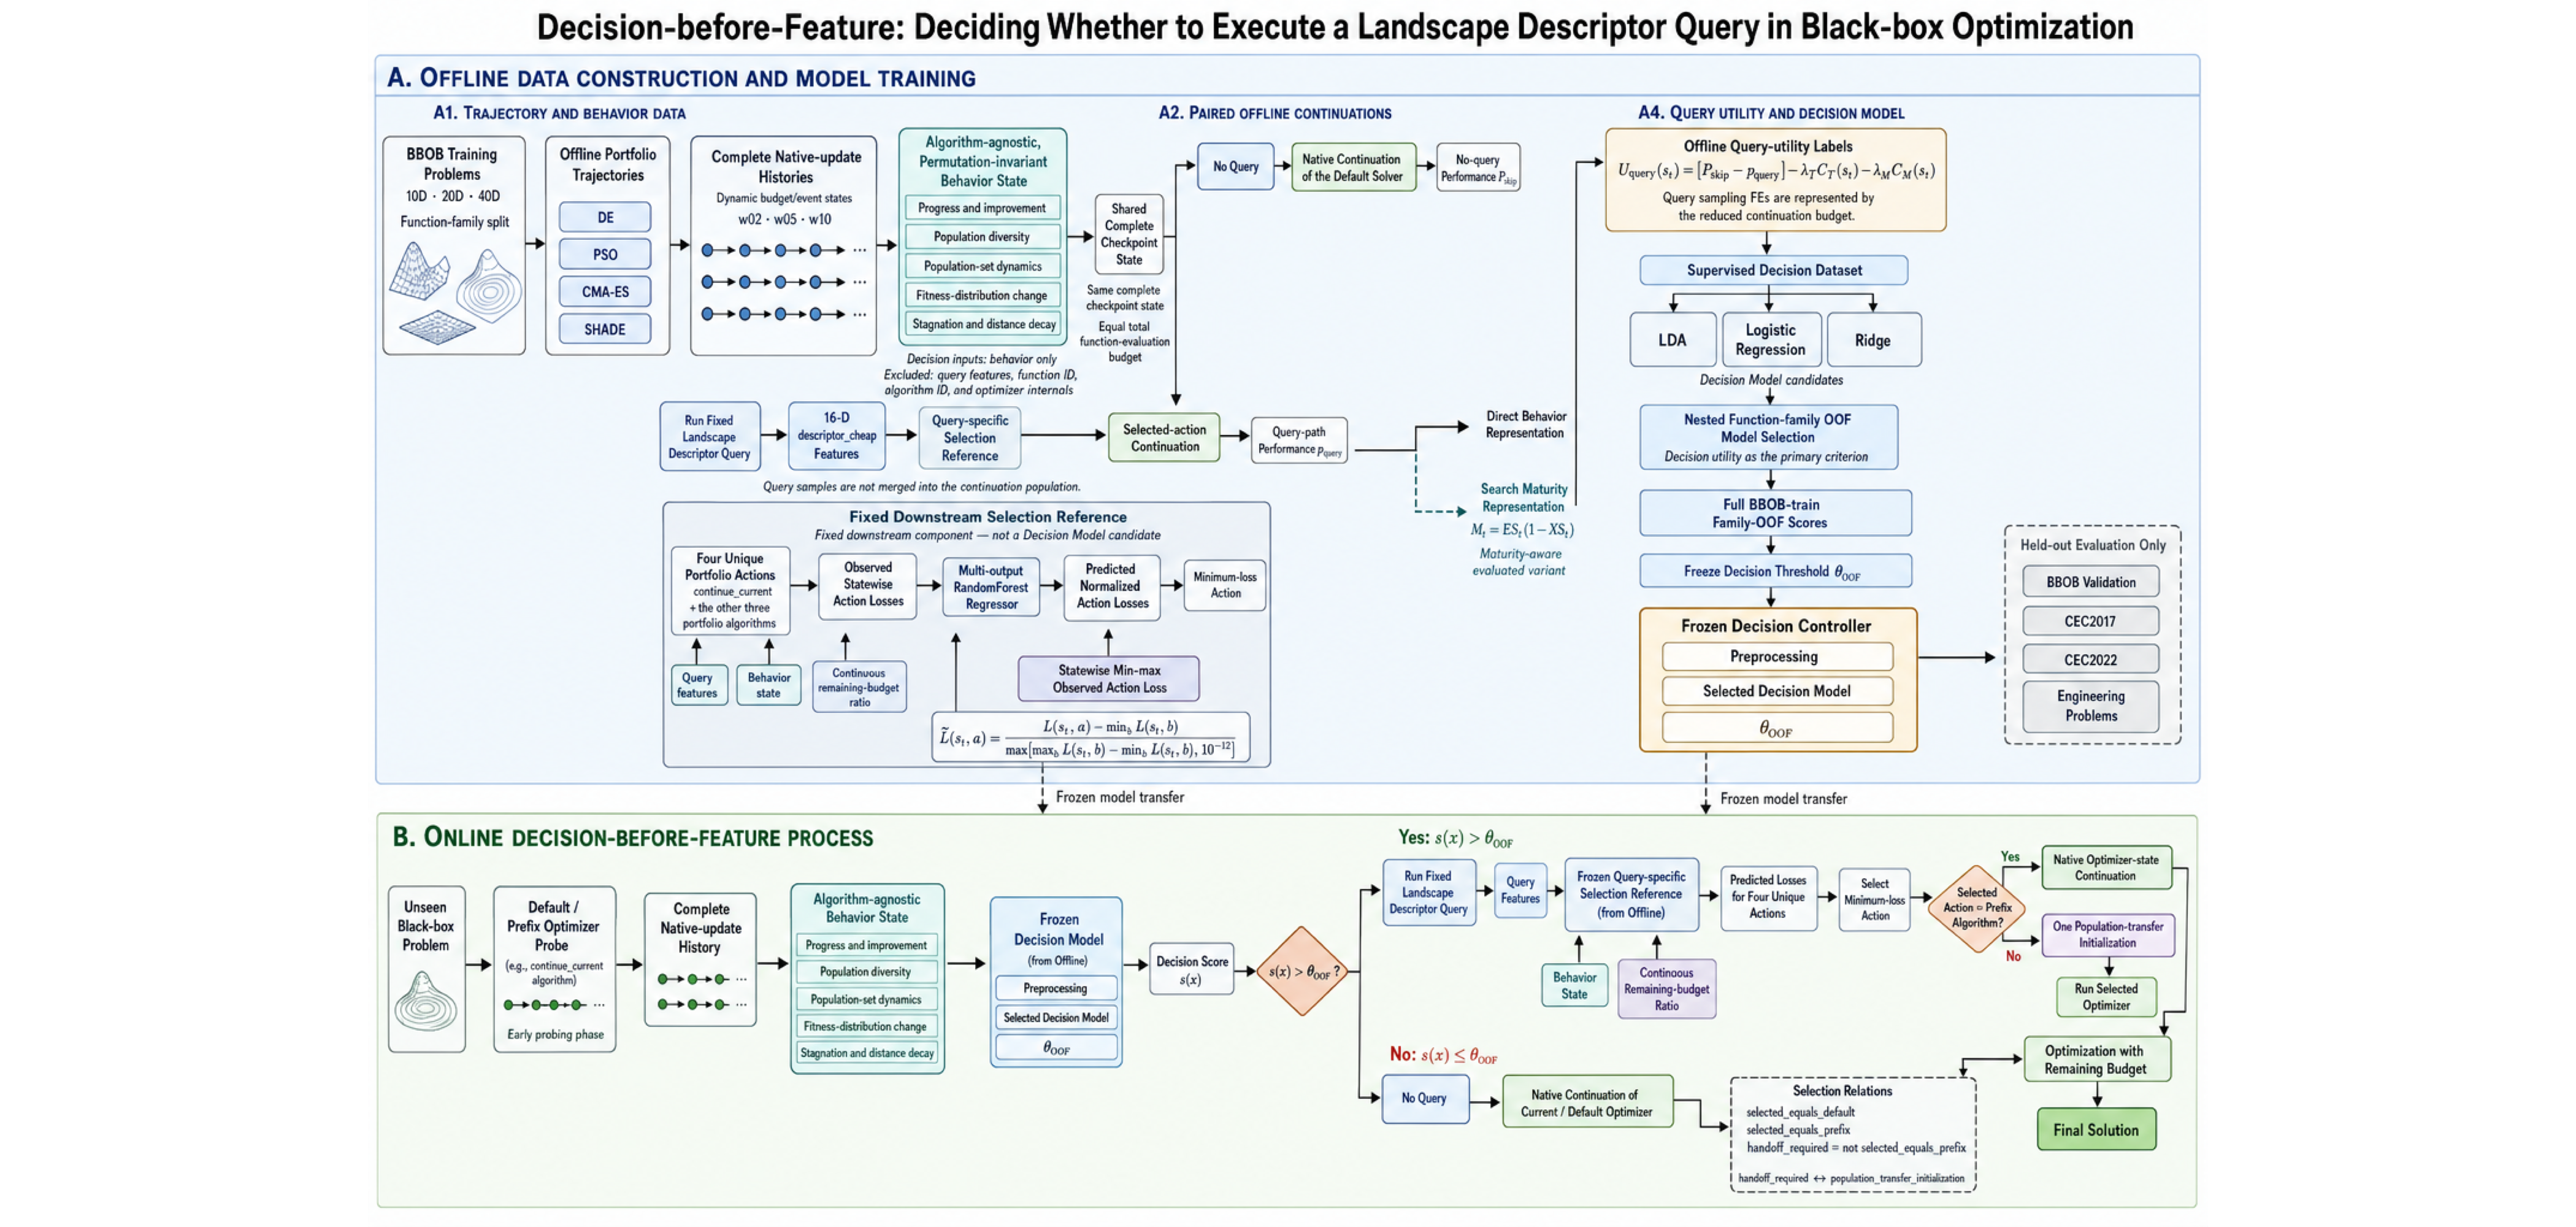
\includegraphics[width=\textwidth]{decision-before-feature-architecture-elsevier.png}
  \caption{Decision-before-Feature protocol.  The upper panel constructs
  state-aligned utility labels and freezes the downstream Selection Reference,
  Decision Model, preprocessing, and threshold using BBOB training families.
  The lower panel applies those frozen components at an online decision
  opportunity.  Query descriptors enter only the downstream Selection
  Reference; the pre-query Decision Model receives algorithm-agnostic behavior.}
  \label{fig:framework}
\end{figure*}

This separation gives the two supervised components different roles.  The \emph{selection reference} operates after query acquisition and may use the query descriptors.  The \emph{decision model} operates before query acquisition and is prohibited from using query descriptors, function identity, dimension, algorithm identity, optimizer-specific parameters, action losses, or best-observed-action diagnostics.

\subsection{Native-state trajectory and window alignment}

For every portfolio optimizer, a complete state contains its population, objective values, best-so-far solution, generation or native-update count, internal dynamic variables, and random-number-generator state.  Restoring this state continues the same optimizer rather than constructing a new run from population values.  This distinction is essential for PSO velocities, CMA-ES distribution parameters, and the adaptation histories of DE and SHADE.

Let $e_t$ be the actual FE count at an accepted state and let $w\in\{0.02,0.05,0.10\}$ be a nominal behavior window.  Among the complete native updates preceding $t$, the anchor is
\begin{equation}
  a(t,w)=\mathop{\arg\max}_{u}
  \left\{e_u:e_u\le e_t-\operatorname{round}(wB)\right\}.
  \label{eq:native-window-anchor}
\end{equation}
For population size $N=40$, the realized span satisfies
\begin{equation}
  \operatorname{round}(wB)
  \le e_t-e_{a(t,w)}
  <\operatorname{round}(wB)+N.
  \label{eq:native-window-bound}
\end{equation}
Rates and slopes use the realized FE-ratio span, not the nominal value.  The realized ratio, FE count, and number of native updates are retained as measurement metadata and are excluded from the decision input.

Behavior vectors are evaluated only at accepted complete-update states.  The
budget milestones, behavior-triggered opportunities, rearming rules, and
per-phase quotas are specified in Section~\ref{sec:experimental-setup};
opportunity labels determine state sampling but are excluded from the Decision
Model.

\subsection{Permutation-invariant behavior representation}

For distance-based population summaries, coordinates are mapped to the unit hypercube using the problem bounds,
\begin{equation}
  \widetilde x_{ij}
  =\frac{x_{ij}-\ell_{pj}}{u_{pj}-\ell_{pj}}.
  \label{eq:unit-cube-scaling}
\end{equation}
This unit-cube convention defines distance normalization.  No correspondence between row $i$ at two checkpoints is assumed.  The current population diversity is the average pairwise distance
\begin{equation}
  D_t=\frac{2}{N(N-1)}
  \sum_{1\le i<j\le N}
  \lVert\widetilde x_i^{(t)}-\widetilde x_j^{(t)}\rVert_2.
  \label{eq:population-diversity}
\end{equation}
For an anchor population and the current population, the empirical assignment distance is
\begin{equation}
  W_t^{(w)}=
  \frac{1}{N}
  \min_{\pi\in S_N}
  \sum_{i=1}^{N}
  \left\lVert
  \widetilde x_i^{(a)}-
  \widetilde x_{\pi(i)}^{(t)}
  \right\rVert_2,
  \label{eq:population-wasserstein}
\end{equation}
and its rate divides Eq.~\eqref{eq:population-wasserstein} by $(e_t-e_a)/B$.  Centroid shift and its rate are computed analogously.  Centroid-shift coherence is the ratio of centroid displacement to $W_t^{(w)}$, clipped to $[0,1]$ and set to zero when the population does not change.  Covariance trace and effective-rank changes use the unit-cube populations.  Current covariance spectral concentration is computed from the raw-coordinate covariance.  For its nonzero eigenvalues $\lambda_j$ and $r=\min(d,N-1)$,
\begin{equation}
  C_t=
  \frac{r\,\sum_j\lambda_j^2/(\sum_j\lambda_j)^2-1}{r-1},
  \label{eq:covariance-concentration}
\end{equation}
with $C_t=0$ for a degenerate covariance or $r\le1$.

Fitness changes use a shift-invariant scale.  Let
\begin{equation}
  I_0=\max\!\left(\operatorname{IQR}(y_{\mathrm{init}}),10^{-12}\right),
  \label{eq:initial-fitness-scale}
\end{equation}
where $y_{\mathrm{init}}$ is the evaluated population immediately after optimizer initialization and before any native update.  Improvement rate over a short window is
\begin{equation}
  IR_t^{(w)}=
  \frac{f_{\mathrm{best}}(a)-f_{\mathrm{best}}(t)}
       {I_0\,(e_t-e_a)/B}.
  \label{eq:improvement-rate}
\end{equation}
Improvement frequency is the proportion of native-update intervals in which best-so-far fitness decreases strictly.  To compare fitness distributions without individual identities, the two endpoint vectors are sorted.  If $y_{(i)}^{(a)}$ and $y_{(i)}^{(t)}$ denote their empirical quantiles, the method records the fraction for which $y_{(i)}^{(a)}-y_{(i)}^{(t)}$ exceeds the numerical strict-improvement tolerance, their mean signed improvement divided by $I_0$ and the realized ratio span, and their mean absolute difference on the same scale.

Stagnation is based on the last strict best-so-far improvement.  With $e_{\mathrm{last}}$ denoting its FE count,
\begin{equation}
  S_t^{(0.10)}=
  \frac{\min\{\max[(e_t-e_{\mathrm{last}})/B,0],0.10\}}{0.10}.
  \label{eq:stagnation}
\end{equation}
Distance decay compares the population's mean unit-cube distance to its current population-best at the long-window endpoints.  Convergence rate is the relative decrease in $D_t$ divided by the realized FE-ratio span.  The reference point in these calculations is the current population-best, not a known global optimum.

The representation borrows the general idea that longitudinal population
summaries can characterize problem--algorithm interaction
\cite{cenikjDynamoRepTrajectoryBasedPopulation2023}, but uses one fixed-dimensional
definition across all four optimizers and predicts query utility rather than a
problem class.  Distance-decay and stagnation semantics are also informed by
behavior-characterization studies
\cite{haywardDeterminingMetaheuristicSimilarity2025,mbassoHowMetaheuristicsExploit2026}.
Measures requiring a known optimum, persistent particle identities, or an
optimizer-specific interaction graph are excluded; in particular, particle-wise
directional entropy is not an input.

The behavior representation has 34 unique outputs: 31 model-eligible variables and three diagnostic-only variables.  The nested groups are summarized in Table~\ref{tab:behavior-groups}.

\begin{table*}[t]
  \caption{Frozen behavior groups used in the feature-group comparison.}
  \label{tab:behavior-groups}
  \centering
  \small
  \begin{tabularx}{\textwidth}{@{}l c X X@{}}
    \toprule
    Group & Count & Added information & Role \\
    \midrule
    T0 & 1 & Actual FE ratio only & Time-only controller \\
    B1 & 19 & Progress, diversity, set and fitness-distribution change, stagnation, convergence, and elite concentration & Core permutation-invariant behavior \\
    B2 & 25 & B1 plus fitness-spread slope, population and elite centroid shifts, covariance trace ratio, covariance effective rank, and diversity recovery & Longitudinal set dynamics \\
    B3 & 31 & B2 plus set-motion proxies and three maturity variables & Primary full input \\
    \bottomrule
  \end{tabularx}
\end{table*}

The raw fitness standard deviation, population-overlap statistic, and best-distance--fitness correlation are diagnostic only.  In particular, the last quantity is close to a local landscape proxy and is excluded from the pre-query model.

\subsection{Operational search-maturity variables}

Search Maturity is an operational, study-specific summary rather than an established convergence measure.  Define
\begin{equation}
\begin{gathered}
  h_+(z)=\frac{\max(z,0)}{1+\max(z,0)},\quad
  h_-(z)=\frac{1}{1+\max(z,0)},\\
  c(z)=\min\{\max(z,0),1\}.
\end{gathered}
\end{equation}
Using the defined behavior variables, exploration stabilization is the mean of
\begin{equation}
  h_+(-\dot D_t),\quad
  h_-(\dot W_t),\quad
  c(C_t),\quad
  c(K_t),
  \label{eq:exploration-stabilization}
\end{equation}
where $\dot D_t$ is the medium-window diversity slope, $\dot W_t$ is the population assignment-distance rate, and $K_t$ is centroid-shift coherence.  Exploitation saturation is the mean of
\begin{equation}
  c(S_t),\quad
  h_-(IR_t),\quad
  h_+(DD_t),\quad
  h_+(CR_t),\quad
  h_-(E_t),
  \label{eq:exploitation-saturation}
\end{equation}
where $DD_t$, $CR_t$, and $E_t$ denote distance decay, convergence rate, and elite-to-population diversity ratio.  The primary maturity variable is
\begin{equation}
  M_t=ES_t(1-XS_t).
  \label{eq:search-maturity}
\end{equation}
The B3 group also contains the bounded linear alternative $c[(ES_t+1-XS_t)/2]$ and an exploration-to-exploitation ratio.  Undefined components remain missing and are handled by training-only median imputation.  Equation~\eqref{eq:search-maturity} is a hypothesis-bearing representation whose utility must be established by the T0--B3 comparison and external evaluation; it is not treated as an independently validated causal mechanism.

\subsection{Query-specific downstream selection reference}

For every eligible shared state, all actions in Eq.~\eqref{eq:state-action-set} are run under the query-adjusted budget.  Because raw objective values vary across problems, each action target is normalized within its state:
\begin{equation}
  \widetilde L(s_t,a)=
  \frac{L(s_t,a)-\min_b L(s_t,b)}
       {\max\!\left(\max_b L(s_t,b)-\min_b L(s_t,b),10^{-12}\right)}.
  \label{eq:selector-target}
\end{equation}
The selection reference predicts the four targets jointly from the 31 B3 behavior variables, the fixed descriptors of the current query, and the continuous remaining-budget ratio $(B-e_t-FE_q)/B$:
\begin{align}
  \widehat{\boldsymbol L}(s_t)
  &=g\!\left(b_t,\phi_q(p),\frac{B-e_t-FE_q}{B}\right),\\
  \widehat a_t&=\arg\min_a\widehat L(s_t,a).
  \label{eq:statewise-selector}
\end{align}
The fixed estimator is a multi-output random-forest regressor with 200 trees, minimum leaf size two, median imputation, and random seed 1701.  BBOB-training rows receive five-fold function-family cross-fitted predictions so that a training utility label never uses a selector fitted on the same family.  The final selector is refitted on all BBOB-training families for BBOB validation and external evaluation.  This selection reference is a downstream experimental component, not the proposed contribution.

For each selected action, three relations distinguish whether it equals the
default, whether it equals the prefix, and whether a handoff is required.
Writing $h_t$ for the handoff indicator, $i_t$ for equality with the prefix,
and $r_t$ for the transition type, these relations satisfy
\begin{equation}
  h_t=\neg \iota_t^{\mathrm{prefix}}
  =\mathbf{1}[r_t=\mathrm{population\ transfer\ initialization}],
  \label{eq:handoff-fields}
\end{equation}
Here $h_t$, $\iota_t^{\mathrm{prefix}}$, and $r_t$ correspond, respectively, to
the reported handoff indicator, equality with the prefix action, and transition
type.  Equality with the default action is reported independently.  These
relations hold by definition for every state, support stratified reporting,
and are not Decision Model inputs.

\subsection{Decision-model selection and threshold fitting}

The active candidates are fixed to (i) linear discriminant analysis with default estimator settings, (ii) logistic regression with $C=1$, balanced class weights, and the L-BFGS solver, and (iii) Ridge regression with $\alpha=1$.  Each candidate is a pipeline containing training-fold median imputation and standard scaling.  LDA and logistic regression fit Eq.~\eqref{eq:query-label}; Ridge fits the continuous primary utility.  These three candidates are compared only with the frozen B3 input group.

Model selection is performed once and is nested entirely within BBOB training.  The outer loop is a five-fold GroupKFold over function families.  Within each outer fit partition, a four-fold family out-of-fold procedure supplies scores used to fit an outer-fold decision threshold.  Candidate quality is the mean decision utility obtained after concatenating all outer holdouts.  Ties are resolved by the prespecified order LDA, logistic regression, then Ridge.  Neither T0, B1, B2 nor BBOB validation contributes to this model-family choice.

After the B3 comparison freezes the model family, that same named estimator
family is used for T0, B1, B2, and B3 with identical samples, family folds,
training-fold preprocessing, and threshold-fitting procedure.  Each input group
fits its threshold only from its own BBOB-training family-OOF scores.  The RQ5
feature-group analysis reports all four prespecified groups; it neither repeats
model-family selection nor selects a feature group from their observed results.
B3 remains the primary deployable representation.

After a model family is selected, a separate five-fold function-family out-of-fold pass over all BBOB-training rows produces one score per row from a model that did not see that row's family.  The deployable threshold is
\begin{equation}
  \tau_{\mathrm{OOF}}
  \in\arg\max_{\tau}
  \sum_i
  \mathbf{1}[z_i^{\mathrm{OOF}}>\tau]U_{q,i}.
  \label{eq:oof-threshold}
\end{equation}
If thresholds yield the same utility sum, the threshold calling fewer rows is preferred.  The selected estimator is then fitted on all BBOB-training families and deployed with the fixed threshold.  BBOB validation is evaluation-only.  The optional score-neighborhood review uses the tenth percentile of $|z_i^{\mathrm{OOF}}-\tau_{\mathrm{OOF}}|$ from BBOB training; it is performed only after model and threshold freezing and gives all comparison policies the same additional opportunities.

At deployment, the default SBS advances natively while the streaming behavior extractor observes complete updates.  At each accepted decision opportunity, the controller evaluates Eq.~\eqref{eq:deployment-decision}.  If the score does not cross the threshold, native optimization continues.  If it crosses, the fixed query is executed once, the downstream selector chooses an action, and the selected continuation consumes the remaining query-adjusted budget.  No subsequent online training or repeated query-type selection is performed.

\section{Experimental setup}
\label{sec:experimental-setup}

\subsection{Research questions and evaluation design}

The empirical study addresses the five prespecified questions in
Table~\ref{tab:research-questions}.  Each question is linked to an estimand, a
comparison set, and uncertainty summaries that respect dependence among states
from the same optimization trajectory and function family.

\begin{table*}[t]
  \caption{Research questions and corresponding evaluation criteria.}
  \label{tab:research-questions}
  \centering
  \small
  \begin{tabularx}{\textwidth}{@{}c Y Y@{}}
    \toprule
    RQ & Question & Evaluation criteria \\
    \midrule
    RQ1 & Statewise value of the primary query & Utility distribution and decomposition; proportion with $U_q\le0$; family-balanced effects and intervals. \\
    RQ2 & Information beyond elapsed budget & Nested training-family OOF selection; paired B3--T0 effects; frozen BBOB-validation evaluation. \\
    RQ3 & End-to-end policy trade-off & Call quality, final performance, FE use, runtime, and paired comparisons with all required policies. \\
    RQ4 & Transport of the frozen procedure & Separate held-out BBOB, CEC2017, CEC2022, and engineering estimates, with coverage and query failures. \\
    RQ5 & Behavioral associations with query value & T0--B3 increments, model-parameter stability, maturity--utility association, and prespecified strata. \\
    \bottomrule
  \end{tabularx}
\end{table*}

\subsection{Internal benchmark and function-family partition}

The internal benchmark is the noiseless BBOB suite.  The training set comprises
functions 1, 2, 3, 4, 6, 7, 8, 10, 11, 12, 15, 16, 17, 18, 20, 21, 22, and 23;
functions 5, 9, 13, 14, 19, and 24 form the held-out validation set.  Functions,
rather than randomly selected transformed instances, define the grouping
variable.  This partition addresses evidence that instance-level splits can
overstate algorithm-selection generalization
\cite{cenikjLandscapeFeaturesSingleobjective2025}.  Both sets use dimensions
$d\in\{10,20,40\}$, instances $1,2,3$, optimizer seeds $1,\ldots,30$, population
size 40, and total budget $B=1000d$.  The portfolio contains DE, PSO, CMA-ES,
and SHADE, giving 54 training and 18 validation function--dimension
combinations.

The single best solver (SBS) is estimated exclusively from terminal outcomes at
$FE=B$.  For each problem--algorithm pair, final best fitness is first averaged
over seeds.  The four algorithms are then ranked within each problem, with
smaller mean fitness preferred and average ranks assigned to ties.  These ranks
are averaged over the training problems; any remaining tie is resolved in the
prespecified order DE, PSO, CMA-ES, SHADE.  Intermediate decision states,
including the last state at or before approximately $0.60B$, do not contribute
to the SBS estimate.

BBOB validation is a held-out internal evaluation set.  It remains untouched
during query selection, preprocessing, model-family selection, input-group
comparison, threshold fitting, and score-neighborhood definition.

\subsection{External benchmarks}

External evaluation is organized as non-pooled, suite-specific analyses.  The
CEC2017 analysis comprises functions 1--29, dimensions 10, 30, and 50, seeds
$1,\ldots,30$, population size 40, and budget $B=1000d$.  The four-algorithm
portfolio and dynamic decision-opportunity protocol are unchanged, and the
controller, downstream selector, imputation values, and threshold are held
fixed at their BBOB-training estimates.

CEC2022 and engineering problems form separate components of RQ4.  Their
problem sets, dimensions, bounds, budgets, success targets, and failure rules
are specified independently of policy-outcome inspection.  For every external
suite, query-extraction failures remain in the coverage denominator rather than
being removed from the analysis.  Missing descriptors may be imputed only with
BBOB-training medians.  Held-out BBOB, CEC2017, CEC2022, and engineering
estimates are reported separately; neither partial coverage nor agreement on a
subset of suites is interpreted as unconditional cross-benchmark transfer.

\subsection{Landscape-query configurations}

Table~\ref{tab:query-configurations} defines the three prespecified queries.
Primary inference concerns \texttt{descriptor\_cheap}; the two \texttt{pflacco}
configurations evaluate dependence on representation and acquisition cost.

\begin{table*}[t]
  \caption{Prespecified landscape-descriptor queries.}
  \label{tab:query-configurations}
  \centering
  \small
  \begin{tabularx}{\textwidth}{@{}l l c c X@{}}
    \toprule
    Query & Sample & FE share & Features & Role \\
    \midrule
    \texttt{descriptor\_cheap} & LHS $50d$ & 5\% & 16 & Primary \\
    \texttt{pflacco\_standard} & Same LHS $50d$ & 5\% & 37 & Configuration robustness \\
    \texttt{pflacco\_broad} & Independent LHS $100d$ & 10\% & 52 & Configuration robustness \\
    \bottomrule
  \end{tabularx}
\end{table*}

The cheap and standard queries use the same evaluated $(X,y)$ sample, yielding
a paired comparison of descriptor representations at a common FE cost.  The
broad query uses an independent $100d$ design.  The standard configuration
comprises PCA, nearest-better clustering, dispersion, information-content, and
ELA-distribution groups.  The broad configuration adds ELA level-set and
sample-derived fitness--distance-correlation groups, while excluding the full
quadratic meta-model group, cell mapping, and feature groups that require
additional objective evaluations.  Query sample points are not inserted into
the optimizer population.  Each query defines a separate downstream selector,
utility target, decision model, threshold, baseline comparison, and external
evaluation; observations from different query identities or FE designs are not
pooled.

\subsection{Dynamic decision opportunities}

Offline label construction and policy evaluation use the same dynamic
budget--event sampling scheme.  Complete native updates are monitored when they
cross a grid from $0.20B$ to $0.60B$ in increments of $0.01B$.  The mandatory
budget milestones are 0.20, 0.22, 0.24, 0.26, 0.28, 0.30, 0.34, 0.38, 0.42,
0.46, 0.50, and 0.60.  Five event types may add decision states: resumed strict
improvement; a stagnation span reaching $0.05B$; an absolute medium-window
covariance-effective-rank change reaching $0.20$; unit-cube elite-centroid
displacement divided by $\sqrt{d}$ reaching $0.05$; and relative diversity
recovery reaching $0.10$.  Covariance-effective-rank-change, elite-migration,
and diversity-recovery events rearm when their respective quantities fall below
$0.10$, $0.025$, and $0.05$.  Stagnation rearms after a new strict best-so-far
improvement, whereas resumed improvement rearms when short-window improvement
frequency returns to zero.

Each complete update that crosses one or more monitor points is evaluated once.
If a crossing includes a milestone, the event is associated with that milestone
and does not consume an event-only quota or spacing anchor.  Otherwise, the most
recent crossed monitor point supplies the nominal location.  Each of the early,
middle, and late phases admits at most two event-only states, with at least
$0.02B$ separation in realized FE ratio.  Suppressed crossings still update
event rearming.  This scheme admits 12--18 states per run, each with unit sample
weight.  The realized $FE/B$ represents elapsed budget and is the sole T0
covariate; exact integer FE aligns shared-state outcomes.  Nominal milestones
and native-update counts describe the sampling process but do not add Decision
Model inputs.

\subsection{Matched states and analysis population}

The analysis pairs all alternatives at an identical complete native state.
For each eligible state, it combines permutation-invariant behavior, the shared
$50d$ and independent $100d$ LHS samples, the three descriptor representations,
and the query-budget-specific outcome of every eligible action.  A trajectory
enters an estimand only when both its complete native history and terminal
outcome satisfy the same state definition.  Query-specific selection
references, utilities, decision models, and policies are estimated from these
matched observations under the family partitions described above.

The primary Decision Model population contains states for which both the prefix
and default algorithm equal the training SBS and the no-query path continues
that optimizer.  States generated from the other prefix algorithms are reserved
for cross-prefix robustness, leave-one-prefix-algorithm-out analysis, and tests
of portability across the four search processes.  They are excluded from
primary model fitting, threshold fitting, and primary result aggregation.

\subsection{Comparison policies}

Eight prespecified comparison roles are retained because they answer different
benchmarking questions.
\begin{itemize}
  \item \textbf{Never Query}: continue the complete SBS state natively and incur no query acquisition cost.
  \item \textbf{Always Query}: execute the fixed query at the first accepted decision opportunity and invoke the same downstream selector used by the proposed policy.
  \item \textbf{Random Analysis}: at each shared opportunity before a call, trigger with probability 0.5.  Thirty independent repetitions use explicit integer random streams.
  \item \textbf{Traditional AAS}: execute the fixed query and apply the same statewise downstream selector, without a preceding Decision-before-Feature controller, consistent with the sample--feature--selector structure of landscape-based selection \cite{guoAutomatedAlgorithmSelection2025}.  Under this definition, it induces the same first-opportunity decision as Always Query.
  \item \textbf{SBS}: use the training-derived static default defined above.  In the primary population, the prefix and default are this same SBS, so its native complete-budget path coincides with Never Query; the separate name preserves its role as the standard algorithm-selection reference rather than introducing another online trajectory.
  \item \textbf{VBS}: use the static, per-problem hindsight choice among complete-budget portfolio outcomes.  It is an upper reference rather than a deployable method and is distinct from the statewise best observed action.
  \item \textbf{Time-only Controller}: use the selected Decision Model family and the same training and threshold procedure as the full controller, with input restricted to $\{FE/B\}$.
  \item \textbf{Decision-before-Feature}: use B3 behavior with the selected model and the threshold estimated from full-training OOF predictions.
\end{itemize}
In the primary population, Never Query and SBS yield the same native terminal
outcome, whereas Always Query and Traditional AAS yield the same
first-opportunity query outcome.  RQ3 therefore reports these roles as
\emph{Never Query / SBS} and \emph{Always Query / Traditional AAS}; each shared
outcome enters summaries and inferential comparisons once.
All online policies share the same accepted decision opportunities, total FE
budget, portfolio, query definition, downstream selector, and
population-transfer rule.  State-only, query-only, and combined statewise
selectors are additionally compared as diagnostics of the downstream selector;
they do not replace the required policy baselines.

\subsection{Evaluation measures}

Decision-model family selection uses nested function-family OOF mean decision
utility.  AUROC, average precision, and Spearman correlation are secondary
score-level measures.  Continuous-utility RMSE is reported only for Ridge;
classification probabilities and discriminant scores are not compared with
continuous utility using RMSE.

Policy-level reporting includes query-call rate, mean decision utility, the
proportion of called states for which $U_q>0$, the fraction of positive-utility
states called, and
\begin{equation}
  \overline U_{\mathrm{decision}}(\pi)
  =\frac{1}{n}\sum_{i=1}^{n}d_{\pi,i}U_q(s_i),
  \label{eq:policy-decision-utility}
\end{equation}
where $d_{\pi,i}$ is the call indicator of query-decision policy $\pi$.  A
skipped state contributes zero, so the Never Query role has zero decision
utility by definition.  The coincident SBS reference role and VBS are not
query-decision policies and therefore remain not applicable for this quantity;
mean observed utility conditional on calling is reported separately.
Positive-utility capture is summarized by
\begin{equation}
  \mathrm{utility\ capture}=
  \frac{\sum_i U_{q,i}\,\mathbf{1}[U_{q,i}>0]\,\mathbf{1}[\widehat d_i=1]}
       {\sum_i U_{q,i}\,\mathbf{1}[U_{q,i}>0]}.
  \label{eq:utility-capture}
\end{equation}
The positive-state capture rate and utility capture in
Eq.~\eqref{eq:utility-capture} are reported separately.  Calls with $U_q\le0$
are summarized by their count, their proportion among calls, and their
accumulated utility loss.

End-to-end endpoints comprise final best objective value or error,
target-based success rate and expected running time (ERT), total and query FEs,
wall-clock time, behavior-extraction time, controller-inference time, query
sampling and descriptor-computation time, downstream-selection latency, and
peak memory.  Success targets are suite specific and are fixed independently
of the observed policy contrasts.  Cost--performance reporting retains all
eight prespecified comparison roles but uses six distinct primary-population
outcomes: five online trajectories, including the two slash-labelled
identities, and the VBS hindsight reference.

\subsection{Statistical analysis}

Repeated states from one trajectory are not treated as independent replicates.
Descriptive summaries include state-level micro-averages and macro-averages
balanced across function families.  Results are also stratified by family,
dimension, phase, and transition type.  Support for the RQ1 statement that a
majority of evaluated states do not benefit from the primary query requires the
95\% lower confidence bound for the relevant proportion to exceed 0.5.  Paired
policy comparisons use nonparametric procedures, including Wilcoxon signed-rank
comparisons and Friedman comparisons with Holm-adjusted follow-ups, at a
prospectively declared aggregation level.
For every endpoint, analytically identical roles enter once; duplicated role
labels add no ranks, paired contrasts, or multiplicity counts.

Equivalence is assessed only against a smallest effect of interest, margin, and
primary procedure fixed before policy outcomes are examined.  Confidence
intervals use a prespecified hierarchical resampling unit and replication
count, and ERT uses suite-specific targets fixed independently of policy
outcomes.  Absence of statistical significance is not interpreted as
equivalence or preservation of optimization performance.

\section{Results}
\label{sec:results}

Results are structured around RQ1--RQ5.  For each question, the corresponding
estimand, family-level uncertainty, and policy or representation contrast are
presented together; held-out BBOB and external-suite estimates are kept
separate.

\subsection{RQ1: How often does the primary query have non-positive net utility?}
\label{sec:results-rq1}

RQ1 concerns the primary low-cost descriptor query under the main cost
weighting, $\lambda_T=1$ and $\lambda_M=0$. Query utility is decomposed into
the observed performance difference, downstream-selector regret, and measured
non-FE query cost. Evaluations consumed by query sampling are already absent
from the continuation budget of the query branch and are therefore not
subtracted again.

\begin{table*}[t]
\caption{State-level utility summary for the primary low-cost descriptor
query. Utility is larger-is-better, whereas final action loss is
smaller-is-better. Function families, rather than individual decision states,
form the independent units for uncertainty quantification.}
\label{tab:rq1-utility}
\centering
\scriptsize
\begin{tabularx}{\textwidth}{@{}l Y c c c c c Y@{}}
\toprule
Analysis stratum & Coverage & States & $\Pr(U_q\leq 0)$ & Mean $U_q$
& Median $U_q$ & Performance difference & Selector regret and query cost \\
\midrule
Overall & All prespecified BBOB-train families, dimensions, and decision
opportunities & -- & -- & -- & -- & -- & -- \\
By split & Separate BBOB-train family-OOF and frozen BBOB-validation estimates
& -- & -- & -- & -- & -- & -- \\
By dimension & 10D, 20D, and 40D & -- & -- & -- & -- & -- & -- \\
By decision stage & Each prespecified dynamic decision opportunity & -- & --
& -- & -- & -- & -- \\
\addlinespace
\multicolumn{8}{l}{\TBD{TBD-RQ1-TAB-01}: numerical estimates and
family-level intervals for all rows.} \\
\bottomrule
\end{tabularx}
\end{table*}

\begin{figure*}[t]
\centering
\fbox{\begin{minipage}{0.90\textwidth}
\centering
\TBD{TBD-RQ1-FIG-01}\\[0.8ex]
Distribution of $U_q$ relative to zero, with function-family-aware uncertainty
and separate views by dimension and actual FE ratio.
\end{minipage}}
\caption{Distributional analysis of utility for the primary query. The zero
reference distinguishes states in which the measured cost-adjusted utility is
non-positive.}
\label{fig:rq1-utility}
\end{figure*}

\paragraph{Statistical analysis.}
\TBD{TBD-RQ1-STAT-01} The family-balanced proportion of states with
$U_q\leq0$ is estimated with function-family-aware uncertainty; paired effects
decompose performance and cost contributions.  State counts are descriptive
and do not serve as independent inferential units.  Equivalence is evaluated
only under the prespecified clustering hierarchy, resample count, smallest
effect of interest, and primary interval or TOST rule.

\paragraph{Answer to RQ1.}
\TBD{TBD-RQ1-CLAIM-01} Whether the primary query has net benefit across the
evaluated decision states is undetermined.  The answer is conditional on the
estimated direction, effect size, interval, and observed state coverage, and is
restricted to the primary query rather than landscape analysis in general.

\FloatBarrier
\subsection{RQ2: Does algorithm-agnostic behavior predict query utility?}
\label{sec:results-rq2}

The active Decision Model candidates are LDA, Logistic Regression, and Ridge.
Their only model-family comparison uses the fixed B3 representation and nested
BBOB-train function-family out-of-fold (OOF) mean decision utility. AUROC,
Average Precision, and Spearman correlation are auxiliary measures, and
continuous-utility RMSE is defined only for Ridge. After this comparison, the
selected estimator family is fitted separately to B3 and T0, with a threshold
derived from the corresponding complete BBOB-train family-OOF scores.
BBOB-validation is evaluation-only and cannot influence preprocessing,
model-family choice, input-group comparison, or threshold estimation.

\begin{table*}[t]
\caption{Decision Model selection and evaluation structure for RQ2. Candidate
models are selected using B3 and nested BBOB-train family-OOF utility only.
The selected estimator family is subsequently fitted separately to B3 and T0;
BBOB-validation is reserved for evaluating these fixed choices without
refitting or reselection.}
\label{tab:rq2-prediction}
\centering
\scriptsize
\begin{tabularx}{\textwidth}{@{}l l Y c c c Y@{}}
\toprule
Analysis & Evaluation population & Estimator and representation
& Mean utility & AUROC / AP & Spearman / RMSE & Inferential role \\
\midrule
Model-family selection & BBOB-train nested family OOF & LDA with B3
& -- & -- & -- & Candidate comparison \\
Model-family selection & BBOB-train nested family OOF & Logistic Regression
with B3 & -- & -- & -- & Candidate comparison \\
Model-family selection & BBOB-train nested family OOF & Ridge with B3
& -- & -- & -- & Candidate comparison \\
\addlinespace
Representation comparison & BBOB-train family OOF & Selected estimator,
B3 versus T0 & -- & -- & -- & Paired B3--T0 effect \\
Frozen evaluation & BBOB-validation & Selected estimator with B3
& -- & -- & -- & Evaluation only \\
Frozen evaluation & BBOB-validation & Selected estimator with T0
& -- & -- & -- & Evaluation only \\
\addlinespace
\multicolumn{7}{l}{\TBD{TBD-RQ2-TAB-01}: model-selection, paired
representation, and frozen-evaluation estimates with family-level intervals.} \\
\multicolumn{7}{l}{RMSE is reported only when the estimator is Ridge; otherwise
it is not applicable. Frozen evaluation includes the paired B3--T0 effect.} \\
\bottomrule
\end{tabularx}
\end{table*}

\begin{figure*}[t]
\centering
\fbox{\begin{minipage}{0.90\textwidth}
\centering
\TBD{TBD-RQ2-FIG-01}\\[0.8ex]
(a) Outer-family OOF decision utility for LDA, Logistic Regression, and Ridge
with B3; (b) paired B3--T0 effects for the selected estimator family on
BBOB-train family-OOF predictions and on the separate frozen
BBOB-validation evaluation. Held-out families are the replication units.
\end{minipage}}
\caption{B3 model-family comparison and fixed B3--T0 evaluation. The
BBOB-validation panel has an evaluation-only role and cannot revise the model
choice made from BBOB-train utility.}
\label{fig:rq2-oof}
\end{figure*}

\paragraph{Statistical analysis.}
\TBD{TBD-RQ2-STAT-01} The paired outer-family BBOB-train OOF comparison for B3,
uses family-level effect sizes, confidence intervals, and Holm-corrected
candidate contrasts.  Conditional on that single model-family selection, the
same estimator family defines the B3--T0 comparison and the separate frozen
BBOB-validation evaluation.  Dependence-aware intervals use the prespecified
resampling unit and replication count; auxiliary score measures and
BBOB-validation cannot supersede the utility-based BBOB-train selection rule.

\paragraph{Answer to RQ2.}
\TBD{TBD-RQ2-CLAIM-01} Whether algorithm-agnostic behavior adds decision value
beyond FE ratio is undetermined and depends on the paired B3--T0 effects and
intervals.  BBOB validation is reserved for evaluating only the frozen models;
an interval that
does not support a stable difference yields an inconclusive answer.

\FloatBarrier
\subsection{RQ3: Does Decision-before-Feature reduce unhelpful query calls?}
\label{sec:results-rq3}

RQ3 retains all eight prespecified comparison roles but reports six distinct
outcome rows in the primary population.  The native path simultaneously
represents Never Query and the training-derived SBS, and the fixed
first-opportunity query path simultaneously represents Always Query and
Traditional AAS.  Random Analysis, the Time-only Controller, and
Decision-before-Feature provide the remaining online trajectories; VBS is a
per-problem hindsight reference.  Slash-labelled pairs are counted once in
summaries and inferential comparisons.  VBS is neither deployable nor the
statewise best observed action.

\begin{table*}[t]
\caption{Equal-budget RQ3 comparison.  Six distinct outcome rows represent all
eight prespecified comparison roles; slash-labelled rows combine definitions
that are analytically identical in the primary population and are counted once.
Panel A combines optimization performance with resource use. Panel B characterizes query-call quality,
including the frequency, within-call rate, and accumulated utility loss of
calls whose observed utility is non-positive.}
\label{tab:rq3-baselines}
\centering
\scriptsize
\begin{tabularx}{\textwidth}{@{}>{\raggedright\arraybackslash}p{0.21\textwidth} Y Y Y Y Y Y@{}}
\toprule
\multicolumn{7}{l}{\textit{Panel A: optimization performance and resource use}} \\
\addlinespace
Outcome row (comparison roles) & Mean decision utility & Final error & Runtime & Total FE & Query FE
& Query-call rate \\
\midrule
Never Query / SBS & 0 / N/A & -- & -- & -- & 0 / N/A & 0 / N/A \\
Always Query / Traditional AAS & -- & -- & -- & -- & -- & -- \\
Random Analysis & -- & -- & -- & -- & -- & -- \\
VBS & N/A & -- & N/A & -- & N/A & N/A \\
Time-only Controller & -- & -- & -- & -- & -- & -- \\
Decision-before-Feature & -- & -- & -- & -- & -- & -- \\
\bottomrule
\end{tabularx}

\vspace{0.8ex}
\begin{tabularx}{\textwidth}{@{}>{\raggedright\arraybackslash}p{0.21\textwidth} Y Y Y Y Y Y@{}}
\toprule
\multicolumn{7}{l}{\textit{Panel B: query-call quality}} \\
\addlinespace
Policy & $U_q\leq0$ calls & Within-call rate & Accumulated utility loss
& Beneficial-state capture & Utility capture & Precision \\
\midrule
Always Query / Traditional AAS & -- & -- & -- & -- & -- & -- \\
Random Analysis & -- & -- & -- & -- & -- & -- \\
Time-only Controller & -- & -- & -- & -- & -- & -- \\
Decision-before-Feature & -- & -- & -- & -- & -- & -- \\
\addlinespace
\multicolumn{7}{@{}>{\raggedright\arraybackslash}p{\textwidth}@{}}{%
\TBD{TBD-RQ3-TAB-01}: numerical estimates and matched family-level intervals
for Panels A and B.} \\
\multicolumn{7}{@{}>{\raggedright\arraybackslash}p{\textwidth}@{}}{%
Never Query / SBS and VBS are omitted from Panel B because call-conditional
quantities are undefined for static references and Never Query makes no calls.} \\
\multicolumn{7}{@{}>{\raggedright\arraybackslash}p{\textwidth}@{}}{%
A slash-labelled row denotes one shared outcome, not an average of two
estimates; it enters each applicable analysis once.} \\
\bottomrule
\end{tabularx}
\end{table*}

\begin{figure*}[t]
\centering
\fbox{\begin{minipage}{0.90\textwidth}
\centering
\TBD{TBD-RQ3-FIG-01}\\[0.8ex]
Final optimization loss, measured runtime, and query-call rate for each
distinct primary-population outcome under equal FE budgets, with function-family-level
uncertainty rather than a frontier based only on point estimates.
\end{minipage}}
\caption{Cost--performance comparison among the equal-budget outcomes.
Coincident comparison roles are shown once.}
\label{fig:rq3-cost-performance}
\end{figure*}

\paragraph{Statistical analysis.}
\TBD{TBD-RQ3-STAT-01} The matched function-family Friedman comparison,
Holm-adjusted paired Wilcoxon contrasts, effect sizes, and confidence intervals
jointly cover mean decision utility as defined in
Eq.~\eqref{eq:policy-decision-utility},
final error, runtime, and both the rate and accumulated cost of calls with
$U_q\leq0$.  The dependence-aware interval construction and equivalence rule
are specified independently of the observed policy differences.
Omnibus and follow-up tests use each distinct applicable outcome once; N/A
roles are omitted endpoint by endpoint, and neither coincident pair is
duplicated.

\paragraph{Answer to RQ3.}
\TBD{TBD-RQ3-CLAIM-01} Whether Decision-before-Feature reduces calls with
non-positive observed utility is undetermined.  A supported answer requires an
interval-supported reduction together with the equal-budget effects on final
optimization performance and runtime; call rate alone is insufficient.

\FloatBarrier
\subsection{RQ4: Does the frozen controller generalize beyond BBOB training families?}
\label{sec:results-rq4}

RQ4 reserves the fully frozen procedure for held-out BBOB-validation families,
CEC2017, CEC2022, and an engineering-problem evaluation to be specified
prospectively. None
of these evaluation sets can refit the Selection Reference, Decision Model,
preprocessing, representation, or OOF utility threshold. Coverage and query
extraction failures are part of the suite-specific evaluation rather than
grounds for silently excluding problems.

\begin{table*}[t]
\caption{Suite-specific evaluation of the frozen controller for RQ4. Coverage
and query-extraction failure rates accompany utility and final optimization
performance so that estimates remain conditional on observed evaluation
coverage. Paired effects compare Decision-before-Feature with Never Query,
Always Query, and the Time-only Controller, in that order.}
\label{tab:rq4-generalization}
\centering
\scriptsize
\begin{tabularx}{\textwidth}{@{}l Y c c c c Y@{}}
\toprule
Evaluation set & Scope & Problem--dimension--seed coverage & Mean utility & Final error
& Query failures & Paired effect and interval \\
\midrule
BBOB-validation & Held-out BBOB function families & -- & -- & -- & -- & -- \\
CEC2017 & Cross-benchmark evaluation & -- & -- & -- & -- & -- \\
CEC2022 & Cross-benchmark evaluation & -- & -- & -- & -- & -- \\
Engineering problems & Problem set to be specified prospectively & -- & -- & -- & -- & -- \\
\addlinespace
\multicolumn{7}{l}{\TBD{TBD-RQ4-TAB-01}: suite-specific coverage,
performance, failure, and matched-effect estimates.} \\
\bottomrule
\end{tabularx}
\end{table*}

\begin{figure*}[t]
\centering
\fbox{\begin{minipage}{0.90\textwidth}
\centering
\TBD{TBD-RQ4-FIG-01}\\[0.8ex]
Suite-specific paired effects and confidence intervals for the frozen
Decision-before-Feature controller relative to Never Query, Always Query, and
the Time-only Controller. Held-out BBOB families are shown separately from
CEC and engineering evaluations.
\end{minipage}}
\caption{Held-out-family and cross-benchmark evaluation of the frozen
controller. Separate panels preserve differences in benchmark scope and data
coverage.}
\label{fig:rq4-generalization}
\end{figure*}

\paragraph{Statistical analysis.}
\TBD{TBD-RQ4-STAT-01} Suite-specific problem- or function-family-level paired
effects, confidence intervals, and multiplicity-adjusted benchmark contrasts
evaluate the frozen policy.  Query-extraction failure sensitivity is separate
from the primary comparison, and heterogeneous effect directions or coverage
preclude a pooled generalization claim.

\paragraph{Answer to RQ4.}
\TBD{TBD-RQ4-CLAIM-01} Held-out BBOB performance and cross-benchmark
generalization are undetermined.  Any eventual answer is suite-specific,
distinguishes BBOB validation from CEC2017, CEC2022, and engineering
evaluations, and remains conditional on query-extraction coverage.

\FloatBarrier
\subsection{RQ5: Which behavior groups are associated with query utility, and when?}
\label{sec:results-rq5}

RQ5 reuses the estimator family selected with B3 in RQ2. That estimator family
is fitted separately to T0, B1, B2, and B3 using identical samples,
function-family splits, train-only preprocessing, and an input-specific
BBOB-train family-OOF threshold. The ablation neither repeats model-family
selection nor changes the primary B3 representation. T0 contains only FE
ratio; B1, B2, and B3 contain the prespecified 19-, 25-, and 31-input
permutation-invariant behavior representations. Coefficients, discriminant
directions, and associations characterize the fitted rule and are not causal
effects.

\begin{table*}[t]
\caption{Prespecified input-group ablation for RQ5. The estimator family is
the one selected with B3 in RQ2 and is fitted separately to each representation.
All groups retain their own BBOB-train family-OOF threshold; the comparison
does not select a replacement for B3.}
\label{tab:rq5-ablation}
\centering
\scriptsize
\begin{tabularx}{\textwidth}{@{}l Y c c c c Y@{}}
\toprule
Group & Added information & Inputs & Mean utility & AUROC / AP
& Spearman / Ridge RMSE & Paired difference from T0 \\
\midrule
T0 & Optimization stage (FE ratio) only & 1 & -- & -- & -- & -- \\
B1 & Progress, diversity, set and fitness-distribution change, stagnation,
convergence, and elite concentration & 19 & -- & -- & -- & -- \\
B2 & B1 plus longitudinal centroid, covariance, fitness-spread, and diversity
recovery summaries & 25 & -- & -- & -- & -- \\
B3 & B2 plus set-motion proxies and the three operational maturity variables
& 31 & -- & -- & -- & -- \\
\addlinespace
\multicolumn{7}{l}{\TBD{TBD-RQ5-TAB-01}: paired family-level ablation
estimates, auxiliary scores, and intervals for all four representations.} \\
\multicolumn{7}{l}{The paired difference from T0 concerns decision utility.
RMSE is not applicable unless the RQ2-selected estimator is Ridge.} \\
\bottomrule
\end{tabularx}
\end{table*}

\begin{figure*}[t]
\centering
\fbox{\begin{minipage}{0.90\textwidth}
\centering
\TBD{TBD-RQ5-FIG-01}\\[0.8ex]
Fold-stable standardized coefficients for Logistic Regression or Ridge, or
standardized discriminant directions for LDA, together with the prespecified
association between behavior-derived search maturity and observed query
utility. Uncertainty and direction changes are separated by family, dimension,
and query configuration.
\end{minipage}}
\caption{Behavior interpretation and search-maturity--utility analysis.
Displayed coefficients or discriminant directions describe the fitted
decision score and do not imply causal effects.}
\label{fig:rq5-interpretation}
\end{figure*}

\paragraph{Statistical analysis.}
\TBD{TBD-RQ5-STAT-01} The paired outer-family effects and
multiplicity-adjusted contrasts compare T0/B1/B2/B3 for the single estimator
family selected in RQ2.  Interpretation also depends on the sign and magnitude
stability of standardized coefficients
or discriminant directions across outer folds and families, Spearman
associations with observed utility, uncertainty around the fitted
maturity--utility curve, and the prespecified dimension and query-configuration
analyses.  Visual shape alone is insufficient evidence of non-monotonicity,
and the ablation cannot repeat model or representation selection.

\paragraph{Answer to RQ5.}
\TBD{TBD-RQ5-CLAIM-01} Whether any behavior increment is informative beyond
optimization stage is undetermined.  Such an interpretation requires agreement
among the paired ablation, parameter or discriminant stability, and held-out
analyses.  Representation- or family-dependent effects instead imply a
correspondingly restricted answer; none can replace B3 through post hoc
selection.

\FloatBarrier
\subsection{Prespecified sensitivity analyses and diagnostics}
\label{sec:results-sensitivity}

These analyses qualify the RQ1--RQ5 conclusions without defining an additional
research question or changing the primary target. Each alternative query
configuration traverses the same complete query-specific sequence of action
selection, utility estimation, decision modelling, and frozen evaluation as
the primary query. The non-primary $\lambda_T$ values do not replace
$\lambda_T=1$. Action-relation indicators define descriptive strata only, and
downstream-selector variants neither enter the Decision Model nor replace the
policy baselines.

\begin{table*}[t]
\caption{Prespecified sensitivity analyses and downstream-selector
diagnostics. Interpretation is restricted to the listed levels and cannot
revise the primary cost weighting, input representation, or policy comparison.}
\label{tab:sensitivity-diagnostics}
\centering
\scriptsize
\begin{tabularx}{\textwidth}{@{}l Y Y Y@{}}
\toprule
Analysis & Prespecified levels & Quantities & Interpretation boundary \\
\midrule
Query configuration & Primary low-cost descriptor query, standard
\textit{pflacco} query, and broad \textit{pflacco} query & Query-specific
action selection, utility, decision-model, policy, and frozen-evaluation
estimates & Agreement indicates robustness only across these three
configurations; disagreement indicates representation or cost dependence \\
$\lambda_T$ sensitivity & $0$, $0.25$, $0.5$, $1$, and $2$, with
$\lambda_M=0$ & Utility distributions, policy summaries, effect sizes, and
intervals & $\lambda_T=1$ remains the primary conclusion basis \\
Action-relation strata & Selected action equals the default action; selected
action equals the prefix algorithm; population handoff is required & Counts,
utility components, selector regret, and policy effects & Descriptive
stratification only; no action-relation indicator enters the Decision Model \\
Downstream-selector inputs & State information only, query descriptors only,
and their combination; remaining budget is included in every variant &
Cross-fitted action-loss regression performance, selected-action loss, and
selector regret & Downstream-selector diagnosis only; these variants are not
Decision Model candidates or substitutes for policy baselines \\
\addlinespace
\multicolumn{4}{l}{\TBD{TBD-SENS-DIAG-01}: estimates and intervals for all
prespecified sensitivity and diagnostic comparisons.} \\
\bottomrule
\end{tabularx}
\end{table*}

\FloatBarrier

\section{Discussion}
\label{sec:discussion}

The present study separates two decisions that are usually collapsed in
feature-based algorithm selection: whether to execute an evaluated fixed
landscape query and, conditional on execution, which portfolio action to use.
This formulation is methodological and does not by itself establish that the
query should be skipped or executed in any empirical regime.

\subsection{When is the evaluated query worth executing?}

\TBD{TBD-DISC-01} The statewise utility distribution has not yet been
estimated.  Its eventual interpretation is conditional on the evaluated query,
utility definition, effect direction, interval, and state coverage, and cannot
be extended from the fixed low-cost query to landscape analysis in general.

\subsection{Information in algorithm-agnostic search behavior}

\TBD{TBD-DISC-02} The RQ2 comparison between T0 and the behavior groups remains
undetermined pending nested BBOB-train family-OOF estimates and frozen
evaluation.  Decision utility, AUROC, Average Precision, Spearman correlation,
and Ridge RMSE support different aspects of the comparison; disagreement among
them precludes a single undifferentiated predictive claim.

\subsection{End-to-end resource and performance trade-offs}

\TBD{TBD-DISC-03} The practical resource--performance trade-off is
undetermined.  Its interpretation requires joint evidence from equal-total-FE
final performance, measured query and inference time, query-call rate, and the
cost of calls with non-positive observed utility.  Fewer calls alone would not
establish better resource-aware optimization.

\subsection{Held-out families and cross-benchmark scope}

\TBD{TBD-DISC-04} Effects on held-out BBOB, CEC2017, CEC2022, and engineering
problems remain unestimated and provide no current evidence of generalization.
Any eventual interpretation is suite-specific; query-extraction failures,
divergent effect directions, or incomplete coverage narrow its scope.

\subsection{Search maturity and behavior interpretation}

\TBD{TBD-DISC-05} The RQ5 ablation, coefficient or discriminant-direction
stability, and maturity--utility association remain unestimated.  Coefficients, discriminant
directions, and correlations have a predictive rather than causal
interpretation; a non-monotonic relationship would require support from its
prespecified fit, interval, and stability analysis.

\subsection{Limitations and validity boundaries}

The primary estimand is query-specific: it concerns
\texttt{descriptor\_cheap}, a 16-dimensional custom low-cost descriptor query.
The prespecified standard and broad \texttt{pflacco} queries can assess
configuration robustness but cannot justify claims
about untested landscape representations. The Selection Reference is a fixed
downstream component rather than a claimed algorithm-selection contribution,
and its selector regret must remain visible when interpreting query utility.
The main Decision Model is trained offline on a BBOB function-family split; the
study does not evaluate online controller training as a primary design.

\TBD{TBD-DISC-06} The empirical limitations remain to be quantified through
trajectory and action-loss coverage, query-extraction failures, family-level
dependence, population-transfer frequency, and sensitivity to the three
prespecified query configurations and utility-cost settings.

\section{Reproducibility}
\label{sec:reproducibility}

\subsection{Software and experimental configuration}

The study uses offline trajectory collection followed by supervised learning.
The experimental specification fixes benchmark membership, dimensions,
instances, optimizer seeds, portfolio composition, population size, FE budgets,
and the dynamic decision-opportunity schedule.
Reporting these elements, together with repetitions, variability, and feature
cost, is particularly important for optimization representations
\cite{cenikjSurveyFeaturesUsed2026}.

The main implementation targets Python 3.12.  The \texttt{pflacco} queries run
in an isolated Python 3.11 environment with \texttt{pflacco==1.2.2},
\texttt{numpy==1.24.3}, \texttt{pandas==2.0.3}, \texttt{scipy==1.10.1}, and
\texttt{scikit-learn==1.2.2}.  The descriptor extractor receives only the
previously evaluated LHS sample.  It neither imports a benchmark nor calls the
objective function, and a failed \texttt{pflacco} feature group is not replaced
by a study-specific substitute.

\subsection{Random streams}

All scientific random streams are constructed from explicit integers through
\texttt{numpy.random.SeedSequence}.  Optimizer streams combine the configured
optimizer seed with integer identifiers for the run and stochastic event.
Query sampling additionally uses integer stream, function, instance, dimension,
and sample-design codes.  Population-transfer initialization receives explicit
function, instance, and event codes.  The Random Analysis repetitions combine a
base seed with problem, dimension, optimizer seed, decision FE, and repetition
indices.  Experimental randomness therefore does not depend on strings or
process-specific hash values.

\subsection{Observation indexing and state alignment}

An observation is uniquely indexed by
\begin{equation}
  k_t=(\mathrm{split},p,\mathcal{F}(p),d,a_t,r,e_t),
  \label{eq:state-key}
\end{equation}
where $p$ uniquely identifies the problem instance, $\mathcal{F}(p)$ is its
function family, $a_t$ is the prefix algorithm,
$r$ is the optimizer seed, and $e_t$ is the exact integer FE count.  This index
aligns trajectories, behavior summaries, action outcomes, selection-reference
predictions, utility labels, and Decision Model observations.  Exact FE, rather
than a rounded budget ratio, identifies a shared state; the corresponding
elapsed-budget covariate is calculated as $e_t/B$.  Nominal milestone ratios and
realized native-window spans describe how the state was sampled but do not
replace exact-FE alignment.

\subsection{Data construction and evaluation dependencies}

Complete native-state trajectories and complete-budget terminal outcomes
define the common analysis population.  Permutation-invariant behavior and the
three fixed descriptor representations are evaluated at matched states, after
which the four query-adjusted actions provide the statewise losses.  Each query
configuration has its own cross-fitted selection reference, utility labels,
Decision Model, threshold, baseline comparison, and held-out evaluation.  Only
trajectories with both a complete native history and a terminal outcome enter
the corresponding estimand.  Query identity, sample design, FE charge, and
descriptor definition jointly identify an analysis condition; in particular,
the 5\% and 10\% acquisition conditions are analyzed separately and are never
pooled.

\subsection{Validity checks}

The validity checks address state continuity, representation invariance, FE
accounting, and information leakage.  For each portfolio optimizer, a restored
complete state is compared with uninterrupted native continuation at matched
checkpoints, including optimizer-specific internal dynamics rather than only
population values.  Independent reordering of population members at every
evaluated BBOB state tests that the 31 Decision Model inputs, three diagnostic
variables, and native-window summaries are permutation invariant.

Query-level checks enforce the three descriptor definitions, the shared sample
for the cheap and standard configurations, four non-duplicated actions,
continuous remaining budget, query-specific FE accounting, the statewise
action-loss transformation, and the utility and selector decompositions.
Feature-group failures remain explicit; undefined individual descriptors are
imputed only from BBOB-training observations.  Model-level checks fit all
preprocessing within the applicable training-family fold, restrict the active
candidates to LDA, Logistic Regression, and Ridge, and exclude BBOB validation
and external suites from model fitting and threshold estimation.  The three
action relations in Eq.~\eqref{eq:handoff-fields} are checked throughout
selection, utility calculation, and policy evaluation.  These procedures assess
implementation validity; they add no observations to RQ1--RQ5.

\subsection{Resource measurement}

FE accounting is exact at the state level:
\begin{align}
  FE_{\mathrm{skip,opt}} &= B-e_t,\\
  FE_{q,\mathrm{opt}} &= B-e_t-FE_q.
\end{align}
Behavior extraction reuses evaluated optimizer states and makes no additional
objective-function calls.  Query time is the sum of sample-evaluation and
feature-computation time.  Selection latency includes state preparation, model
inference, and action choice.  Prediction time is measured separately for the
T0 and B3 controllers.

All resource measurements use one fixed hardware and software environment.
Processor, operating system, Python environments, thread count, batch size,
cache state, and the peak-memory procedure accompany the estimates.  Timings
are decomposed into behavior extraction, T0 and B3 inference, query sampling,
descriptor computation, downstream selection, and total wall time.
\TBD{TBD-REPRO-RESOURCE-01}

\subsection{Recomputation of estimands}

The state-level release retains the quantities needed to recompute every term
in Eq.~\eqref{eq:query-utility} and Eq.~\eqref{eq:selector-decomposition},
including the observed losses, normalization and cost terms, selected action,
and three action relations.  Model summaries are reconstructed from
training-family fold assignments, nested and full-training OOF scores,
thresholds, and held-out predictions.  Policy summaries are reconstructed from
the trigger state, query decision, selected action, transition mode, FE use,
timing components, and terminal loss.

Equivalence is interpreted only relative to margins and procedures fixed
before policy-outcome inspection.  Held-out BBOB and each external suite are
analyzed separately with every train-derived component frozen.  These
provisions define reproducibility and do not themselves constitute evidence of
held-out or cross-benchmark transfer.

\section{Conclusion}
\label{sec:conclusion}

This work formulates analysis selection as a decision that precedes the
execution of a prespecified fixed landscape query. The proposed offline workflow
links full-state optimizer trajectories, permutation-invariant behavior states,
statewise observed action losses, a fixed Selection Reference, and a supervised
Decision Model while preserving equal total FE budgets. These design elements
define the evaluation; they do not substitute for the empirical
evidence required by RQ1--RQ5.

\TBD{TBD-CONC-RQ1} Whether the primary query has non-positive utility in a
statistically supported subset of states remains undetermined; the required
effect size, interval, and query-specific scope are not yet available.

\TBD{TBD-CONC-RQ2} Whether algorithm-agnostic behavior predicts query utility
beyond FE ratio alone remains undetermined pending nested function-family OOF
evidence and frozen evaluation.

\TBD{TBD-CONC-RQ3} Effects on calls with non-positive utility, mean decision
utility, measured runtime, and equal-budget final optimization performance
relative to the prespecified policies remain undetermined.

\TBD{TBD-CONC-RQ4} No conclusion is currently supported for held-out BBOB
families or any external suite.  BBOB-validation, CEC, and engineering-problem
generalization remain unverified pending the corresponding estimates and
coverage analyses.

\TBD{TBD-CONC-RQ5} Behavior-group and search-maturity associations remain
undetermined and, when estimated, have a descriptive interpretation conditional
on the prespecified representations.

The contribution is limited to the prespecified query configurations. Consistent
evidence from three prespecified configurations
would support configuration robustness, not a universal conclusion about all
landscape analysis methods or representations.


\bibliographystyle{cas-model2-names}
\bibliography{references}

\end{document}
